%% Run LaTeX on this file several times to get Table of Contents,
%% cross-references, and citations.

\documentclass[11pt]{book}
\usepackage{gvv-book}
\usepackage{gvv}
%\usepackage{Wiley-AuthoringTemplate}
\usepackage[sectionbib,authoryear]{natbib}% for name-date citation comment the below line
%\usepackage[sectionbib,numbers]{natbib}% for numbered citation comment the above line

%%********************************************************************%%
%%       How many levels of section head would you like numbered?     %%
%% 0= no section numbers, 1= section, 2= subsection, 3= subsubsection %%
\setcounter{secnumdepth}{3}
%%********************************************************************%%
%%**********************************************************************%%
%%     How many levels of section head would you like to appear in the  %%
%%				Table of Contents?			%%
%% 0= chapter, 1= section, 2= subsection, 3= subsubsection titles.	%%
\setcounter{tocdepth}{2}
%%**********************************************************************%%

%\includeonly{ch01}
\makeindex

\begin{document}

\frontmatter
%%%%%%%%%%%%%%%%%%%%%%%%%%%%%%%%%%%%%%%%%%%%%%%%%%%%%%%%%%%%%%%%
%% Title Pages
%% Wiley will provide title and copyright page, but you can make
%% your own titlepages if you'd like anyway
%% Setting up title pages, type in the appropriate names here:

\booktitle{Signal Processing }

\subtitle{Through GATE}

\AuAff{G. V. V. Sharma}


%% \\ will start a new line.
%% You may add \affil{} for affiliation, ie,
%\authors{Robert M. Groves\\
%\affil{Universitat de les Illes Balears}
%Floyd J. Fowler, Jr.\\
%\affil{University of New Mexico}
%}

%% Print Half Title and Title Page:
%\halftitlepage
\titlepage

%%%%%%%%%%%%%%%%%%%%%%%%%%%%%%%%%%%%%%%%%%%%%%%%%%%%%%%%%%%%%%%%
%% Copyright Page

\begin{copyrightpage}{2024}
%Title, etc
\end{copyrightpage}

% Note, you must use \ to start indented lines, ie,
% 
% \begin{copyrightpage}{2004}
% Survey Methodology / Robert M. Groves . . . [et al.].
% \       p. cm.---(Wiley series in survey methodology)
% \    ``Wiley-Interscience."
% \    Includes bibliographical references and index.
% \    ISBN 0-471-48348-6 (pbk.)
% \    1. Surveys---Methodology.  2. Social 
% \  sciences---Research---Statistical methods.  I. Groves, Robert M.  II. %
% Series.\\

% HA31.2.S873 2004
% 001.4'33---dc22                                             2004044064
% \end{copyrightpage}

%%%%%%%%%%%%%%%%%%%%%%%%%%%%%%%%%%%%%%%%%%%%%%%%%%%%%%%%%%%%%%%%
%% Only Dedication (optional) 

%\dedication{To my parents}

\tableofcontents

%\listoffigures %optional
%\listoftables  %optional

%% or Contributor Page for edited books
%% before \tableofcontents

%%%%%%%%%%%%%%%%%%%%%%%%%%%%%%%%%%%%%%%%%%%%%%%%%%%%%%%%%%%%%%%%
%  Contributors Page for Edited Book
%%%%%%%%%%%%%%%%%%%%%%%%%%%%%%%%%%%%%%%%%%%%%%%%%%%%%%%%%%%%%%%%

% If your book has chapters written by different authors,
% you'll need a Contributors page.

% Use \begin{contributors}...\end{contributors} and
% then enter each author with the \name{} command, followed
% by the affiliation information.

% \begin{contributors}
% \name{Masayki Abe,} Fujitsu Laboratories Ltd., Fujitsu Limited, Atsugi, Japan
%
% \name{L. A. Akers,} Center for Solid State Electronics Research, Arizona State University, Tempe, Arizona
%
% \name{G. H. Bernstein,} Department of Electrical and Computer Engineering, University of Notre Dame, Notre Dame, South Bend, Indiana; formerly of
% Center for Solid State Electronics Research, Arizona
% State University, Tempe, Arizona 
% \end{contributors}

%%%%%%%%%%%%%%%%%%%%%%%%%%%%%%%%%%%%%%%%%%%%%%%%%%%%%%%%%%%%%%%%
% Optional Foreword:

%\begin{foreword}
%\lipsum[1-2]
%\end{foreword}

%%%%%%%%%%%%%%%%%%%%%%%%%%%%%%%%%%%%%%%%%%%%%%%%%%%%%%%%%%%%%%%%
% Optional Preface:

%\begin{preface}
%\lipsum[1-1]
%\prefaceauthor{}
%\where{place\\
% date}
%\end{preface}

% ie,
% \begin{preface}
% This is an example preface.
% \prefaceauthor{R. K. Watts}
% \where{Durham, North Carolina\\
% September, 2004}

%%%%%%%%%%%%%%%%%%%%%%%%%%%%%%%%%%%%%%%%%%%%%%%%%%%%%%%%%%%%%%%%
% Optional Acknowledgments:

%\acknowledgments
%\lipsum[1-2]
%\authorinitials{I. R. S.}  

%%%%%%%%%%%%%%%%%%%%%%%%%%%%%%%%
%% Glossary Type of Environment:

% \begin{glossary}
% \term{<term>}{<description>}
% \end{glossary}

%%%%%%%%%%%%%%%%%%%%%%%%%%%%%%%%
%\begin{acronyms}
%\acro{ASTA}{Arrivals See Time Averages}
%\acro{BHCA}{Busy Hour Call Attempts}
%\acro{BR}{Bandwidth Reservation}
%\acro{b.u.}{bandwidth unit(s)}
%\acro{CAC}{Call / Connection Admission Control}
%\acro{CBP}{Call Blocking Probability(-ies)}
%\acro{CCS}{Centum Call Seconds}
%\acro{CDTM}{Connection Dependent Threshold Model}
%\acro{CS}{Complete Sharing}
%\acro{DiffServ}{Differentiated Services}
%\acro{EMLM}{Erlang Multirate Loss Model}
%\acro{erl}{The Erlang unit of traffic-load}
%\acro{FIFO}{First in - First out}
%\acro{GB}{Global balance}
%\acro{GoS}{Grade of Service}
%\acro{ICT}{Information and Communication Technology}
%\acro{IntServ}{Integrated Services}
%\acro{IP}{Internet Protocol}
%\acro{ITU-T}{International Telecommunication Unit -- Standardization sector}
%\acro{LB}{Local balance}
%\acro{LHS}{Left hand side}
%\acro{LIFO}{Last in - First out}
%\acro{MMPP}{Markov Modulated Poisson Process}
%\acro{MPLS}{Multiple Protocol Labeling Switching}
%\acro{MRM}{Multi-Retry Model}
%\acro{MTM}{Multi-Threshold Model}
%\acro{PASTA}{Poisson Arrivals See Time Averages}
%\acro{PDF}{Probability Distribution Function}
%\acro{pdf}{probability density function}
%\acro{PFS}{Product Form Solution}
%\acro{QoS}{Quality of Service}
%\acro{r.v.}{random variable(s)}
%\acro{RED}{random early detection}
%\acro{RHS}{Right hand side}
%\acro{RLA}{Reduced Load Approximation}
%\acro{SIRO}{service in random order}
%\acro{SRM}{Single-Retry Model}
%\acro{STM}{Single-Threshold Model}
%\acro{TCP}{Transport Control Protocol}
%\acro{TH}{Threshold(s)}
%\acro{UDP}{User Datagram Protocol}
%\end{acronyms}

\setcounter{page}{1}

\begin{introduction}
This book provides solutions to signal processing problems in GATE.

\end{introduction}

\mainmatter

\chapter{Harmonics}
\chapter{Filters}
\chapter{ Z-transform}
\chapter{Systems}
\begin{enumerate}[label=\thechapter.\arabic*,ref=\thechapter.\theenumi]

\item Consider a unity-gain negative feedback system consisting of the plant $G\brak{s}$  and a proportional-integral controller. Let the proportional gain and integral
gain be 3 and 1, respectively. For a unit step reference input, the final values of the
controller output and the plant output, respectively, are
\begin{align}
    G\brak{s} = \frac{1}{\brak{s-1}} \notag
\end{align}\hfill (GATE EE 2023)\\
\solution 
\iffalse
\let\negmedspace\undefined
\let\negthickspace\undefined
\documentclass[journal,12pt,twocolumn]{IEEEtran}
\usepackage{cite}
\usepackage{amsmath,amssymb,amsfonts,amsthm}
\usepackage{algorithmic}
\usepackage{graphicx}
\usepackage{textcomp}
\usepackage{xcolor}
\usepackage{txfonts}
\usepackage{listings}
\usepackage{enumitem}
\usepackage{mathtools}
\usepackage{float}
\usepackage{gensymb}
\usepackage{comment}
\usepackage[breaklinks=true]{hyperref}
\usepackage{tkz-euclide} 
\usepackage{listings}
\usepackage{gvv}                                        
\def\inputGnumericTable{}                                 
\usepackage[latin1]{inputenc}                                
\usepackage{color}                                            
\usepackage{array}          
\usetikzlibrary{positioning, arrows.meta}
\usepackage{longtable}                                       
\usepackage{calc}                                             
\usepackage{multirow}                                         
\usepackage{hhline}                                           
\usepackage{ifthen}                                           
\usepackage{lscape}
\usepackage{amsmath}
\newtheorem{theorem}{Theorem}[section]
\newtheorem{problem}{Problem}
\newtheorem{proposition}{Proposition}[section]
\newtheorem{lemma}{Lemma}[section]
\newtheorem{corollary}[theorem]{Corollary}
\newtheorem{example}{Example}[section]
\newtheorem{definition}[problem]{Definition}
\newcommand{\BEQA}{\begin{eqnarray}}
\newcommand{\EEQA}{\end{eqnarray}}
\newcommand{\define}{\stackrel{\triangle}{=}}
\theoremstyle{remark}
\newtheorem{rem}{Remark}
\begin{document}

\bibliographystyle{IEEEtran}
\title{GATE-EE-Q14}
\author{EE23BTECH11015 - DHANUSH V NAYAK$^{*}$% <-this % stops a space
}
\maketitle
\newpage
\bigskip
\renewcommand{\thefigure}{\arabic{figure}}
\renewcommand{\thetable}{\theenumi}
\textbf{Question:}Consider a unity-gain negative feedback system consisting of the plant $G\brak{s}$  and a proportional-integral controller. Let the proportional gain and integral
gain be 3 and 1, respectively. For a unit step reference input, the final values of the
controller output and the plant output, respectively, are
\begin{align}
    G\brak{s} = \frac{1}{\brak{s-1}} \notag
\end{align} \hfill (GATE EE 2023)
\solution 
\fi
\begin{table}[H]
\centering
\renewcommand\thetable{1}
\setlength{\extrarowheight}{9pt}
\resizebox{0.5\textwidth}{!}{
\begin{tabular}{|c|c|c|}
\hline
\textbf{Parameter} & \textbf{Description} & \textbf{Value} \\ \hline
$K_{p}$ & Proportional Gain & 3  \\ \hline
$K_{i}$ & Integral Gain &1 \\ \hline
$r\brak{t}$& Reference Input & $u\brak{t}$ \\ \hline 
$w\brak{t}$& Controller Output & $?$ \\ \hline 
$y\brak{t}$ & Plant Output & $?$ \\ \hline
$e\brak{t}$ & Error Input & $r\brak{t}-y\brak{t}$ \\ \hline
\end{tabular}}
\caption{Parameter Table}
\label{tab:gate_ee_Q14}
\end{table}

From the\figref{fig:gate_ee_Q14_blockdiagram}:
\begin{align}
    E\brak{s}&= U\brak{s} - Y\brak{s}\label{eq:gate_ee_Q14.1}\\
W\brak{s} &= 3E\brak{s} + \frac{1}{s}E\brak{s}\label{eq:gate_ee_Q14.2}\\
    Y\brak{s} &= G\brak{s}W\brak{s} \label{eq:gate_ee_Q14.3}
\end{align}
Some results:
\begin{align}
    tx\brak{t} &\system{L} -\frac{d{X\brak{s}}}{ds} \label{eq:laplace_diff_prop}\\
    e^{-at}x\brak{t} &\system{L} X\brak{s+a}\label{eq:laplace_timeshifting_prop}
\end{align}
By using \eqref{eq:laplace_diff_prop} and \eqref{eq:laplace_timeshifting_prop}:
\begin{align}
    e^{-t}u\brak{t} &\system{L} \frac{1}{s+1} ,  Re\brak{s}>-1 \label{eq:gate_ee_Q14result.1}\\
    t e^{-t}u\brak{t} &\system{L} \frac{1}{\brak{s+1}^2},  Re\brak{s}>-1 
 \label{eq:gate_ee_Q14result.2}
\end{align}

\begin{figure}[H]
    \resizebox{0.9\textwidth}{!}{\tikzset{
    block/.style = {draw, fill=white, rectangle, minimum height=3em, minimum width=3em},
    tmp/.style  = {coordinate}, 
    minus/.style= {draw, fill=white, circle, node distance=1cm, append after command={\pgfextra \draw ($(\tikzlastnode.center) + (-0.15,0)$) -- ($(\tikzlastnode.center) + (0.15,0)$) node[above] {$-$}; \endpgfextra}},
    plus/.style= {draw, fill=white, circle, node distance=1cm, append after command={\pgfextra \draw ($(\tikzlastnode.center) + (-0.15,0)$) -- ($(\tikzlastnode.center) + (0.15,0)$) node[above] {$+$}; \endpgfextra}},
    input/.style = {coordinate},
    output/.style= {coordinate},
    pinstyle/.style = {pin edge={to-,thin,black}}
}


\begin{tikzpicture}[auto, node distance=2cm,>=latex]
    \node [input, name=rinput] (rinput) {};
    \node [minus, right of=rinput] (sum1) {};
    
    \node [block, right of=sum1] (controller) {$k_{p}=3$};
    \node [block, above of=controller, node distance=2cm] (up) {$\frac{k_{i}}{s}=\frac{3}{s}$};
    
    \node [plus, right of=controller, node distance=2cm] (sum2) {};
    \node [block, right of=sum2, node distance=3.5cm] (system) {$G\brak{s}=\frac{1}{\brak{s-1}}$};
    \node [output, right of=system, node distance=2cm] (output) {};
    \node [tmp, below of=controller] (tmp1) {$H(s)$};

    \draw [->] (rinput) -- node[below]{$r\brak{t}$} (sum1);
    \draw [->] (sum1) -- node[name=z,anchor=north,fill=white,circle,inner sep=1pt]{$e\brak{t}$} (controller);
    \draw [->] (controller) -- (sum2);
    \draw [->] (sum2) -- node[above, pos=0.8]{$w\brak{t}$} (system);
    \draw [->] (system) -- node [name=y] {$y\brak{t}$} (output);
    \draw [->] (z) |- (up);
    \draw [->] (up) -| (sum2);
    \draw [->] (y) |- (tmp1) -| (sum1);
\end{tikzpicture}
}
    \caption{Block Diagram of System}
    \label{fig:gate_ee_Q14_blockdiagram}
\end{figure}
\begin{enumerate}
\item \textbf{Plant Output:}\\
From \eqref{eq:gate_ee_Q14.1} , \eqref{eq:gate_ee_Q14.2} and \eqref{eq:gate_ee_Q14.3}:
\begin{align}
    Y\brak{s} &=  \frac{3s+1}{s\brak{s+1}^2} ,  Re\brak{s}>-1 \label{eq:Y(s)}
\end{align}
Final Value Theorem:    
\begin{align}
    \lim_{t \to \infty} x\brak{t}&= \lim_{s \to 0} sX\brak{s}\label{eq:finalval_thm}
\end{align}
Using \eqref{eq:finalval_thm} on Y\brak{s}:
\begin{align}
     \lim_{t \to \infty} y\brak{t}&= \lim_{s \to 0} sY\brak{s}\\
                            &= 1
\end{align}

Taking partial fraction of \eqref{eq:Y(s)} :
\begin{align}
    Y\brak{s} &= \frac{1}{s} + \frac{2}{\brak{s+1}^2} - \frac{1}{s+1}
\end{align}
Using \eqref{eq:gate_ee_Q14result.1} and \eqref{eq:gate_ee_Q14result.2}:
\begin{align}
    \therefore y\brak{t} &= u\brak{t}+ 2t e^{-t}u\brak{t} - e^{-t}u\brak{t}
\end{align}
\item \textbf{Controller Output:}\\
From \eqref{eq:gate_ee_Q14.2}
\begin{align}
     W\brak{s} &= \frac{3}{s} + \frac{1}{s^2} - Y\brak{s}\brak{3+\frac{1}{s}}
\end{align}
Substituting \eqref{eq:Y(s)}
\begin{align}
    W\brak{s} &= \frac{\brak{s-1}\brak{3s+1}}{s\brak{s+1}^2} ,  Re\brak{s}>-1 \label{eq:W(s)}
\end{align}
Using \eqref{eq:finalval_thm} on W\brak{s}
\begin{align}
     \lim_{t \to \infty} w\brak{t}&= \lim_{s \to 0} sW\brak{s}\\
                            &= -1
\end{align}
Taking partial fraction of equation\eqref{eq:W(s)} :
\begin{align}
    W\brak{s} &= -\frac{1}{s} - \frac{4}{\brak{s+1}^2} + \frac{4}{s+1}
\end{align}
Using equations \eqref{eq:gate_ee_Q14result.1} and \eqref{eq:gate_ee_Q14result.2} and taking inverse lapalace transform:
\begin{align}
    w\brak{t} &= -u\brak{t}-4t e^{-t}u\brak{t} +4 e^{-t}u\brak{t}
\end{align}

\begin{figure}[H]
    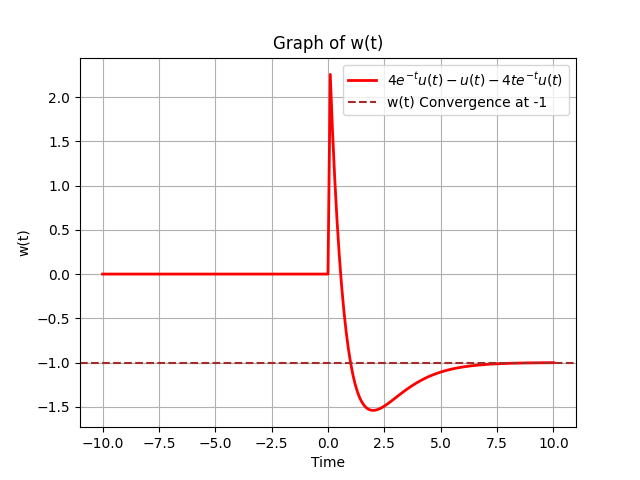
\includegraphics[width=1\columnwidth]{2023/EE/14/figs/Plot of w(t).png}
    \caption{$w\brak{t}$ converges at -1.}
    \label{fig:w_t}
\end{figure}

\begin{figure}[H]
    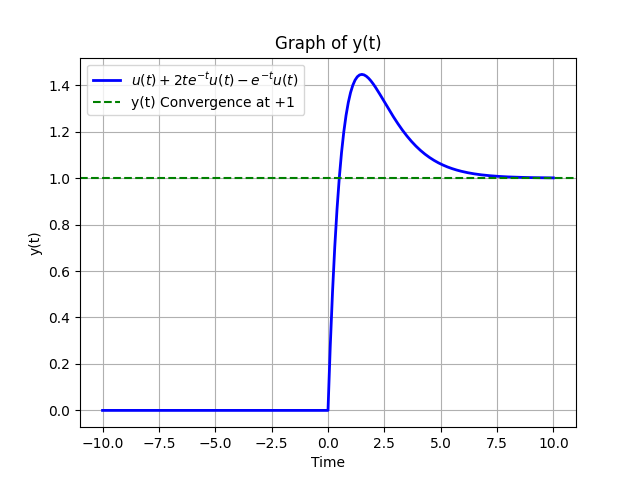
\includegraphics[width=1\columnwidth]{2023/EE/14/figs/Plot of y(t).png}
    \caption{$y\brak{t}$ converges at +1}
    \label{fig:y_t}
\end{figure}

\end{enumerate}
%\end{document}


\newpage

\item Level \brak{h} in a steam boiler is controlled by manipulating the flow rate \brak{F} of the break-up(fresh) water using a proportional \brak{P} controller. The transfer function between the output and the manipulated input is   \\
$$ \frac{h\brak{s}}{F\brak{s}}=\frac{0.25\brak{1-s}}{s\brak{2s+1}} $$   \\
The measurement and the valve transfer functions are both equal to 1. A process engineer wants to tune the controller so that the closed loop response gives the decaying oscillations under the servo mode. Which one of the following is the CORRECT value of the controller gain to be used by the engineer? \\
\begin{enumerate}[label=(\alph*)]
    \item $0.25$
    \item $2$
    \item $4$
    \item $6$
\end{enumerate} \hfill{GATE CH 2023} \\

\solution
 \iffalse
\let\negmedspace\undefined
\let\negthickspace\undefined
\documentclass[journal,12pt,twocolumn]{IEEEtran}
\usepackage{cite}
\usepackage{amsmath,amssymb,amsfonts,amsthm}
\usepackage{algorithmic}
\usepackage{graphicx}
\usepackage{textcomp}
\usepackage{xcolor}
\usepackage{txfonts}
\usepackage{listings}
\usepackage{enumitem}
\usepackage{mathtools}
\usepackage{gensymb}
\usepackage{comment}
\usepackage[breaklinks=true]{hyperref}
\usepackage{tkz-euclide} 
\usepackage{listings}
\usepackage{gvv}                                        
\def\inputGnumericTable{}                                 
\usepackage[latin1]{inputenc}                                
\usepackage{color}                                            
\usepackage{array}                                            
\usepackage{longtable}                                       
\usepackage{calc}                                             
\usepackage{multirow}                                         
\usepackage{hhline}                                           
\usepackage{ifthen}                                           
\usepackage{lscape}

\newtheorem{theorem}{Theorem}[section]
\newtheorem{problem}{Problem}
\newtheorem{proposition}{Proposition}[section]
\newtheorem{lemma}{Lemma}[section]
\newtheorem{corollary}[theorem]{Corollary}
\newtheorem{example}{Example}[section]
\newtheorem{definition}[problem]{Definition}
\newcommand{\BEQA}{\begin{eqnarray}}
\newcommand{\EEQA}{\end{eqnarray}}
\newcommand{\define}{\stackrel{\triangle}{=}}
\theoremstyle{remark}
\newtheorem{rem}{Remark}
\begin{document}
\parindent 0px
\bibliographystyle{IEEEtran}
\title{GATE: CH - 45.2023}
\author{EE22BTECH11219 - Rada Sai Sujan$^{}$% <-this % stops a space
}
\maketitle
\newpage
\bigskip
\section*{Question}
Level \brak{h} in a steam boiler is controlled by manipulating the flow rate \brak{F} of the break-up(fresh) water using a proportional \brak{P} controller. The transfer function between the output and the manipulated input is   \\
$$ \frac{h\brak{s}}{F\brak{s}}=\frac{0.25\brak{1-s}}{s\brak{2s+1}} $$   \\
The measurement and the valve transfer functions are both equal to 1. A process engineer wants to tune the controller so that the closed loop response gives the decaying oscillations under the servo mode. Which one of the following is the CORRECT value of the controller gain to be used by the engineer? \\
\begin{enumerate}[label=(\alph*)]
    \item $0.25$
    \item $2$
    \item $4$
    \item $6$
\end{enumerate} \\
\solution
\fi

\begin{table}[ht]
    \centering
    \begin{tabular}{|p{2cm}|p{6cm}|}
    \hline
    PARAMETER & DESCRIPTION \\ \hline
    $$G_c$$ & Proportional controller's transfer function \\ \hline
    $$G_f$$ & Valve transfer function \\ \hline
    $$G_p$$ & Process transfer function   \\ \hline
    $$G_M$$ & Measurement transfer function \\ \hline 
    $$G\brak{s}$$ & Open loop transfer function \\ \hline
    $$T\brak{s}$$ & Transfer function of system \\ \hline
\end{tabular}

    \caption{PARAMETER TABLE 1}
    \label{tab:ch.45.1}
\end{table} \\
\begin{figure}[ht]
    \centering
    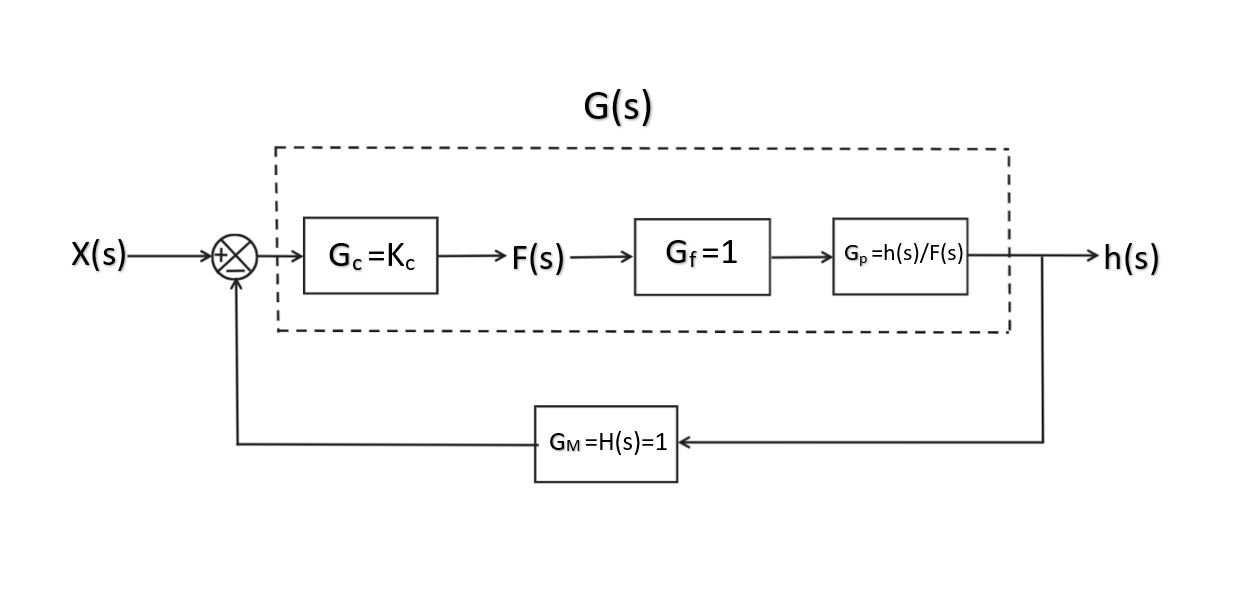
\includegraphics[width=\columnwidth]{2023/CH/45/figs/k.png}
    \caption{Closed loop Block diagram}
    \label{fig:ch.45.1}
\end{figure}    \\
Closed loop signal transfer function of the above block diagram can be given by,
\begin{align}
     T\brak{s} &= \frac{G\brak{s}}{1+G\brak{s}H\brak{s}}    
\end{align}
From \figref{fig:ch.45.1} and \tabref{tab:ch.45.1}
for a unit impulse, $X\brak{s}=1$ \\
\begin{align}
    h\brak{s} &= T\brak{s}\times X\brak{s}   \\
    h\brak{s} &= \frac{\brak{1-s}K_c}{8s^2 + \brak{4-K_c}s + K_c}  \\
    \implies h\brak{s} &= \frac{\brak{1-s}K_c}{8\brak{s-s_1}\brak{s-s_2}}  \label{eq:ch.45.4}
\end{align}
Where,
\begin{align}
    s_1 &= \frac{\brak{K_c-4}}{16} + \sqrt{\brak{\frac{K_c-4}{16}}^2 - \frac{K_c}{8}}  \\
    s_2 &= \frac{\brak{K_c-4}}{16} - \sqrt{\brak{\frac{K_c-4}{16}}^2 - \frac{K_c}{8}} 
\end{align}
From \eqref{eq:ch.45.4} we get,
\begin{align}
    h\brak{s} &= \frac{K_c}{8\brak{s_1-s_2}}\brak{\frac{1-s_1}{s-s_1}-\frac{1-s_2}{s-s_2}}
\end{align}
Now taking the inverse laplace transform we have,
\begin{align}
    h\brak{t} &= \frac{K_c}{8\brak{s_1-s_2}} \left [\brak{1-s_1}e^{s_1t}-\brak{1-s_2}e^{s_2t} \right ]u\brak{t}  \\
    \implies h\brak{t} &= e^{\frac{K_c-4}{16}}\brak{A_1e^{\sqrt{\brak{\frac{K_c-4}{16}}^2 - \frac{K_c}{8}}} - A_2e^{-\sqrt{\brak{\frac{K_c-4}{16}}^2 - \frac{K_c}{8}}}}u\brak{t}    
\end{align}
Where,
\begin{align}
    A_1 &= \frac{K_c}{8} \brak{\frac{1-s_1}{s_1-s_2}}    \\
    A_2 &= \frac{K_c}{8} \brak{\frac{1-s_2}{s_1-s_2}}    
\end{align}
Now applying the condition for underdamped oscillations,
\begin{align}
    \brak{\frac{K_c-4}{16}}^2 - \frac{K_c}{8} < 0    \\
    \implies K_c \in \brak{20-\sqrt{384} , 20+\sqrt{384}}   \label{eq:ch.45.13}
\end{align}
For the system to be stable,
\begin{align}
    \frac{K_c-4}{8}&<0   \\
    \implies K_c&<4 	\label{eq:ch.45.15}
\end{align}
From \eqref{eq:ch.45.13} and \eqref{eq:ch.45.15}
\begin{align}
    &K_c \in \brak{0.4,4}    \label{eq:ch.45.16}
\end{align}
\eqref{eq:ch.45.16} represents the $ROC$,$(R_e\{s\}<0)$
\begin{align}
    \implies &K_c=2
\end{align}
\begin{figure}[htbp]
    \centering
    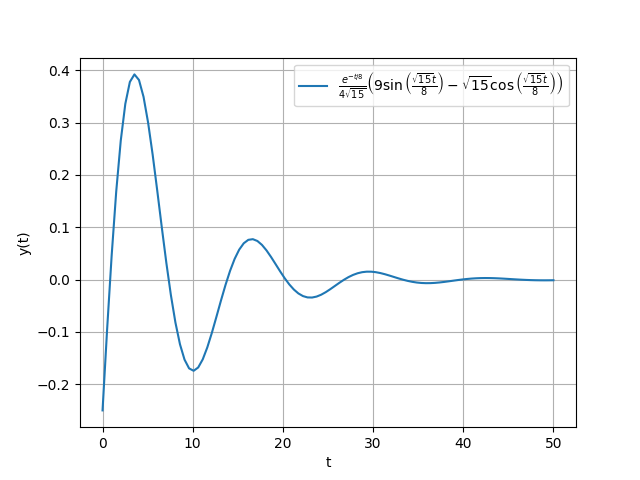
\includegraphics[width=\columnwidth]{2023/CH/45/figs/b.png}
    \caption{y\brak{t} $vs$ t graph}
    \label{fig:ch.45.2}
\end{figure}     

\newpage
\item \iffalse
\let\negmedspace\undefined
\let\negthickspace\undefined
\documentclass[journal,12pt,twocolumn]{IEEEtran}
\usepackage{cite}
\usepackage{amsmath,amssymb,amsfonts,amsthm}
\usepackage{algorithmic}
\usepackage{graphicx}
\usepackage{textcomp}
\usepackage{xcolor}
\usepackage{txfonts}
\usepackage{listings}
\usepackage{enumitem}
\usepackage{mathtools}
\usepackage{gensymb}
\usepackage{comment}
\usepackage[breaklinks=true]{hyperref}
\usepackage{tkz-euclide} 
\usepackage{listings}
\usepackage{gvv}                                        
\def\inputGnumericTable{}                                 
\usepackage[latin1]{inputenc}                                
\usepackage{color}                                            
\usepackage{array}                                            
\usepackage{longtable}                                       
\usepackage{calc}                                             
\usepackage{multirow}                                         
\usepackage{hhline}                                           
\usepackage{ifthen}                                           
\usepackage{lscape}
\usepackage{placeins}
\usepackage{xparse}


\newtheorem{theorem}{Theorem}[section]
\newtheorem{problem}{Problem}
\newtheorem{proposition}{Proposition}[section]
\newtheorem{lemma}{Lemma}[section]
\newtheorem{corollary}[theorem]{Corollary}
\newtheorem{example}{Example}[section]
\newtheorem{definition}[problem]{Definition}
\newcommand{\BEQA}{\begin{eqnarray}}
\newcommand{\EEQA}{\end{eqnarray}}
\newcommand{\define}{\stackrel{\triangle}{=}}
\theoremstyle{remark}
\newtheorem{rem}{Remark}

\graphicspath{ {./figs/} } 

\begin{document}

\bibliographystyle{IEEEtran}
\vspace{3cm}

\Large\title{GATE ME 30}
\large\author{EE23BTECH11032 - Kaustubh Parag Khachane $^{*}$% <-this % stops a space
}
\maketitle
\newpage
\bigskip

\renewcommand{\thefigure}{\theenumi}
\renewcommand{\thetable}{\theenumi}
\large\textbf{Question GATE ME 30} :\\
The figure shows a block of mass m = 20 kg attached to a pair of identical linear springs, each having a spring constant k = 1000 N/m. The block oscillates on a frictionless horizontal surface. Assuming free vibrations, the time taken by the block to complete ten oscillations is \rule{1cm}{0.15mm} seconds . (Rounded off to two decimal places) Take $\pi$ = 3.14. \\ \hfill(GATE ME 2023)

\begin{figure}[!ht]
\centering
\begin{center}
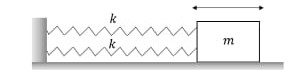
\includegraphics[width=\columnwidth]{2023/ME/30/figs/questiondiagram.jpg}
\end{center}
%\caption{Diagram for GATE ME Question 30}
\end{figure}

\solution\\
\fi
\begin{table}[!ht] 
\centering
\setlength{\extrarowheight}{8pt}
\begin{tabular}{|l|l|l|}
    \hline
    \textbf{Parameter} & \textbf{Description} & \textbf{Value} \\
    \hline
     $k_i$ & spring constant & 1000 N/m \\
    \hline
     m & mass of block & 20Kg \\
    \hline
    k & Equivalent spring constant& $k_1 + k_2$ (parallel)\\
    \hline
     $\omega_n$ & Natural frequency & $\sqrt{\frac{k}{m}}$ \\
    \hline
    T & Time period of an oscillation & $\frac{2\pi}{\omega_n}$ \\
    \hline
    x & Displacement of block & \\
    \hline
    a & Acceleration of block & $\frac{d^2x}{dt^2}$\\
    \hline
    F & Force on block & \\
    \hline
    A & Amplitude of oscillation & x\brak{0}\\
    \hline
  \end{tabular}
  \vspace{4mm}
 \caption{Parameter Table}
 \label{tab:table0_me30_2023}
\end{table}

\begin{align}
    F &= ma \\
    F &= -kx \\
    \implies ma + kx &= 0\\
    \therefore m\frac{d^2x}{dt^2} + kx &= 0\label{eq:eq1_me30_2023}
\end{align}
The Laplace transform of the terms is ,
\begin{align}
    x & \system{\mathcal{L}} X\brak{s}\label{eq:eq3_me30_2023}\\
    \frac{d^2x}{dt^2} & \system{\mathcal{L}} s^2 X\brak{s} - sx\brak{0} - \dot{x}\brak{0}\label{eq:eq2_me30_2023}
\end{align}
Using equation \eqref{eq:eq3_me30_2023} and \eqref{eq:eq2_me30_2023} in equation \eqref{eq:eq1_me30_2023},
\begin{align}
    &m\brak{s^2 X\brak{s} - sx\brak{0} - \dot{x}\brak{0}} + kX\brak{s} = 0\\
    &ms^2X\brak{s} -msA + kX\brak{s} = 0
\end{align}
\begin{align}
    X\brak{s} &= \frac{msA}{ms^2 + k} \\
     &= \frac{sA}{s^2 + \frac{k}{m}} \label{eq:eq4_me30_2023}
\end{align}
The inverse Laplace transform of such terms is given by,
\begin{align}
    \frac{s}{s^2 + a^2} \system{\mathcal{L^{ -}}} cos\brak{at}u\brak{t}
\end{align}
$\therefore$ the inverse Laplace of \eqref{eq:eq4_me30_2023} is,
\begin{align}
    x\brak{t} = Acos\brak{\sqrt{\frac{k}{m}}t} \label{eq:eq5_me30_2023}
\end{align}
From equation \eqref{eq:eq5_me30_2023} and \tabref{tab:table0_me30_2023} ,the time to complete one oscillation is,
\begin{align}
    T_n &= \frac{2\pi}{\sqrt{\frac{k}{m}}}\\
    &= \frac{\pi}{5}\label{eq:eq6_me30_2023}
\end{align}
$\therefore$ the time required for 10 oscillations is ,
\begin{align}
    10T_n &= 2\pi\\
    &= 6.28 s
\end{align}
\begin{figure}[!ht]
\centering
\begin{center}
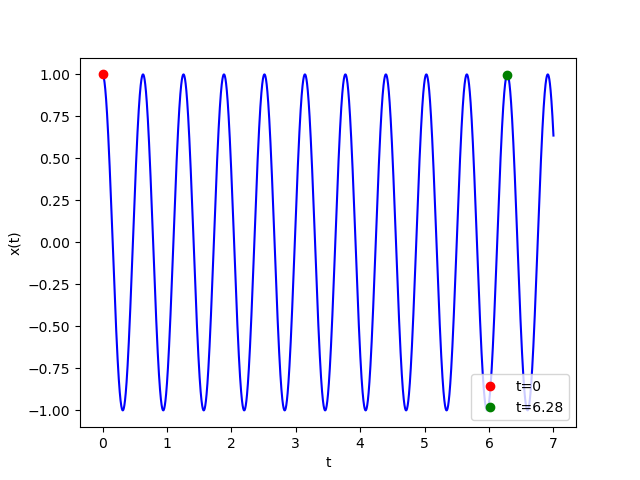
\includegraphics[width=\columnwidth]{2023/ME/30/figs/Figure_1.png}
\end{center}
\caption{Plot of $x\brak{t}$}
\end{figure}


\item A system has transfer function
 \[\frac{Y(s)}{X(s)}=\frac {s-\pi}{s+\pi}\]
 let $u(t)$ be the unit step function.The input $x(t)$ that results in a steady-state output $y(t)=sin(\pi t)$ is \underline{\quad}.\hfill (GATE IN 2023)\\
 \solution
 \newpage
 \item The state equation of a second order system is \\
$ \dot{\bm{x}}(t) = A\bm{x}(t)$, \quad $\bm{x}(0)$ is the initial condition. \\
Suppose $\lambda_1$ and $\lambda_2$ are two distinct eigenvalues of $A$, and $\nu_1$ and $\nu_2$ are the corresponding eigenvectors. For constants $\alpha_1$ and $\alpha_2$, the solution, $\bm{x}(t)$, of the state equation is \\
\begin{enumerate}[label=(\Alph*)]
\item $\sum_{i=1}^{2} \alpha_ie^{\lambda_it}\bf{\nu}_i$
\item $\sum_{i=1}^{2} \alpha_ie^{2\lambda_it}\bf{\nu}_i$
\item $\sum_{i=1}^{2} \alpha_ie^{3\lambda_it}\bf{\nu}_i$
\item $\sum_{i=1}^{2} \alpha_ie^{4\lambda_it}\bf{\nu}_i$
\end{enumerate}
\hfill{GATE 2023 EC Question 43} \\
\newpage
\item Consider the complex function
\[ f(z) = \frac{z^{2}\sin z}{(z-\pi)^4} \]
At \( z = \pi \), which of the following options is (are) correct?
\begin{enumerate}[label=\textbf{\arabic*.}, font=\bfseries, align=left]
    \item[(A)] The order of the pole is 4 
    \item[(B)] The order of the pole is 3 
    \item[(C)] The residue at the pole is \( \frac{\pi}{6} \)
    \item[(D)] The residue at the pole is \( \frac{2\pi}{3} \)
\end{enumerate}
\hfill (GATE PH 2023)
\newpage
 \item
 A buoy of virtual mass $30$ kg oscillates in a fluid medium as a single degree of
freedom system. If the total damping in the system is set as $188.5$ N-s/m, such
that the oscillation just ceases to occur, then the natural period of the system is
\rule{1cm}{0.15mm} s (round off to one decimal place)
\hfill(GATE MN 2023 question 63)\\
\item 
Which of the following statement(s) is/are true?
\begin{enumerate}[label=(\alph*)]
	\item If an LTI system is causal, it is stable.
	\item A discrete time LTI system is causal if and only if its response to a step input $u[n]$ is 0 for $n < 0$.
	\item If a discrete time LTI system has an impulse response $h[n]$ of finite duration the system is stable.
	\item If the impulse response $0 < |h[n]| < 1$ for all $n$, then the LTI system is stable.
\end{enumerate}
\hfill (GATE EE 2023 question 27)\\
\solution
\newpage

\item The outlet concentration $C_A$ of a plug flow reactor (PFR) is controlled by manipulating the inlet concentration $C_{A0}$.The following transfer function describes the dynamics of this PFR.
\begin{align*}
    \frac{C_{A}(s)}{C_{A0}(s)}=e^{-(\frac{V}{F})(k+s)}
\end{align*}
In the above question, V=1$m^3$,F=0.1$m^3$$min^{-1}$ and k=0.5$min^{-1}$.The measurement and valve transfer functions are both equal to 1.The ultimate gain, defined as the proportional controller gain that produces sustained oscillations, for this system is\\ \hfill{(GATE 2023 CH 61)}\\
\solution
\item For the block diagram shown in the figure, the transfer function $\frac{Y\brak{s}}{R\brak{s}}$ is \\
\begin{figure}[H]
    {\tikzset{
    block/.style = {draw, fill=white, rectangle, minimum height=1cm, minimum width=1cm},
    plus/.style= {draw, fill=white, circle, node distance=1cm, append after command={\pgfextra \draw ($(\tikzlastnode.center) + (-0.15,0)$) -- ($(\tikzlastnode.center) + (0.15,0)$) node[above] {$+$}; \endpgfextra}},
    input/.style = {coordinate},
    output/.style = {coordinate}
}


\begin{tikzpicture}[node distance=2cm,>=latex]
    \node [input] (input) at (0,0){};
    \node [block] (block1) at (2,-2){$2$};
    \node [block] (block2) at (6,-2){$3$};
    \node [plus] (sum1) at (2,-4) {};
    \node [plus] (sum2) at (6,-4){};
    \node [block] (block3) at (4,-4) {$\frac{1}{s}$};
    \node [output] (output) at (8,-4){};
    \node [block] (block4) at (4,-6){1};
    
    \draw (input) -- node[above]{$R\brak{s}$} (2,0) to (6,0);
    \draw [->] (6,0) -- (block2);
    \draw [->] (2,0) -- (block1);
    \draw [->] (block1) -- (sum1);
    \draw [->] (sum1) -- (block3);
    \draw [->] (block3) -- (sum2);
    \draw [->] (sum2) -- node[above]{$Y\brak{s}$}(output);
    \draw [->] (block2) -- (sum2);
    \draw (7,-4) to (7,-6);
    \draw [->] (7,-6) -- (block4);
    \draw (block4) to (2,-6);
    \draw [->] (2,-6) to (sum1);  
\end{tikzpicture}
}
    \caption{Block diagram}
    \label{fig:gate_ee_Q12_blockdiagram}
\end{figure}
\hfill (GATE EE 2023)\\
\solution
\newpage

\item  In the following block diagram, $R(s)$ and $D(s)$ are two inputs. The output Y(s) is expressed as $Y(s) = G_1(s)R(s) + G_2(s)D(s).$\\
$G_1(s)$ and $G_2(s)$ are given by \hfill{GATE 2023 EC Question 42}\\
\begin{figure}[htbp]
\centering
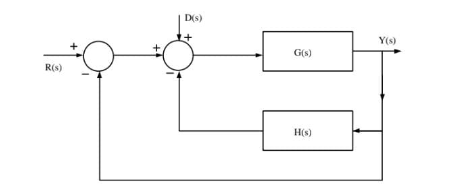
\includegraphics[width=\columnwidth]{2023/EC/42/figs/gate.png}
\end{figure}
\solution
\newpage

\item In the table shown below, match the signal type with its spectral characteristics.\hfill(gate EC 29)\\

\begin{table}[ht]
    \centering
    \def\arraystretch{2.5}
    \begin{tabular}{|c|c|}
\hline
Signal Type & Spectral Characterstics \\
\hline
$\brak{i}$  Continuous, aperiodic & \brak{a} Continuous, aperiodic\\
\hline
$\brak{ii}$ Continuous, periodic & \brak{b} Continuous, periodic \\
\hline
$\brak{iii}$ Discrete, aperiodic & \brak{c} Discrete, aperiodic\\
\hline
$\brak{iii}$ Discrete, periodic & \brak{c} Discrete, periodic\\
\hline
\end{tabular}

\end{table}
\solution
\newpage


\item
The impulse response of an LTI system is $h\brak{t}$= $\delta\brak{t}$+0.5$ \delta\brak{t-4}$, where $\delta\brak{t}$ is continuous-time unit impulse signal.If the input signal $x(t)=\cos\brak{\frac{7\pi t}{4}}$,the output is\hfill(GATE IN 2023)\\
\solution
\newpage
\end{enumerate}

\chapter{Sequences}
\begin{enumerate}[label=\thechapter.\arabic*,ref=\thechapter.\theenumi]

\item Consider the discrete time signal $x\sbrak{n} = u\sbrak{-n+5} - u\sbrak{n+3}$, where
\[u\sbrak{n} = 
\begin{cases}
    1;n\geq0\\
    0;n<0
\end{cases}
\]
The smallest n for which $x\sbrak{n} = 0$ is?
\\ \solution
\iffalse
\let\negmedspace\undefined
\let\negthickspace\undefined
\documentclass[journal,12pt,twocolumn]{IEEEtran}
\usepackage{cite}
\usepackage{amsmath,amssymb,amsfonts,amsthm}
\usepackage{algorithmic}
\usepackage{graphicx}
\usepackage{textcomp}
\usepackage{xcolor}
\usepackage{txfonts}
\usepackage{listings}
\usepackage{enumitem}
\usepackage{mathtools}
\usepackage{gensymb}
\usepackage{comment}
\usepackage[breaklinks=true]{hyperref}
\usepackage{tkz-euclide} 
\usepackage{listings}
\usepackage{gvv}                                        
\def\inputGnumericTable{}                                 
\usepackage[latin1]{inputenc}                                
\usepackage{color}                                            
\newtheorem{theorem}{Theorem}[section]
\usepackage{array}                                            
\usepackage{longtable}                                       
\usepackage{calc}                                             
\usepackage{multirow}                                         
\usepackage{hhline}                                           
\usepackage{ifthen}                                           
\usepackage{lscape}
\newtheorem{problem}{Problem}
\newtheorem{proposition}{Proposition}[section]
\newtheorem{lemma}{Lemma}[section]
\newtheorem{corollary}[theorem]{Corollary}
\newtheorem{example}{Example}[section]
\newtheorem{definition}[problem]{Definition}
\newcommand{\BEQA}{\begin{eqnarray}}
\newcommand{\EEQA}{\end{eqnarray}}
\newcommand{\define}{\stackrel{\triangle}{=}}
\theoremstyle{remark}
\newtheorem{rem}{Remark}
\begin{document}
\bibliographystyle{IEEEtran}
\vspace{3cm}
\title{GATE: IN/28}
\author{EE23BTECH11040 - Manoj Kumar Ambatipudi$^{*}$% <-this % stops a space
}
\maketitle
\newpage
\bigskip
\renewcommand{\thefigure}{\theenumi}
\renewcommand{\thetable}{\theenumi}
\textbf{QUESTION:}
Consider the discrete time signal $x\sbrak{n} = u\sbrak{-n+5} - u\sbrak{n+3}$, where
\[u\sbrak{n} = 
\begin{cases}
    1;n\geq0\\
    0;n<0
\end{cases}
\]
The smallest n for which $x\sbrak{n} = 0$ is?\\
\textbf{Solution:}
\fi
From \figref{IN/28/fig1}, the minimum value of $n$ is given as 
\begin{align}
    n = -3
\end{align}
\begin{figure}[h!]
\renewcommand\thefigure{1}
    \centering
    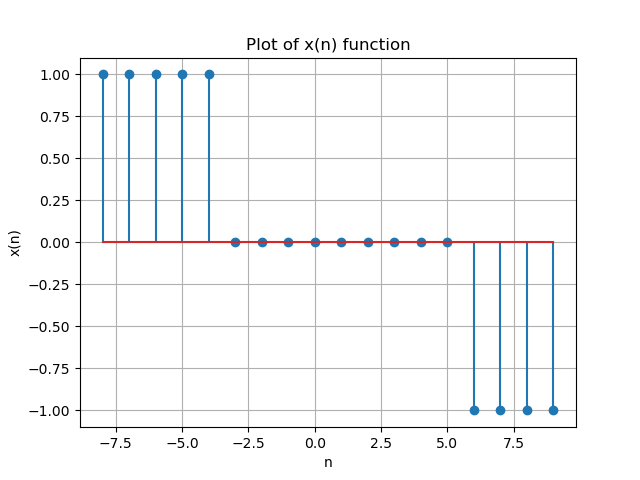
\includegraphics[width=1.0\columnwidth]{2023/IN/28/figs/fig_1.png}
    \caption{Plot of function $x\brak{n}$ taken from python3}
    \label{IN/28/fig1}
\end{figure}


\newpage
\item Two sequences $x_1\sbrak{n} $ and $ x_2 \sbrak{n}$ are described as follows:
\begin{align}
x_1\sbrak{0} = x_2\sbrak{0} = 1\\
x_1\sbrak{1} = x_2\sbrak{2} = 2\\
x_1\sbrak{2} = x_2\sbrak{1} = 1
\end{align}
$x_1\sbrak{n} = x_2\sbrak{n} = 0$ for all $n<0$ and $n>2$\\
\\
If $x\sbrak{n}$ is obtained by convoluting $x_1\sbrak{n}$ with $x_2\sbrak{n}$, which of the following equations is/are TRUE?\\
\\
(A) $x\sbrak{2} = x\sbrak{3}$\\
\\
(B) $x\sbrak{1} = 2$\\
\\
(C) $x\sbrak{4} = 3$\\
\\
(D) $x\sbrak{2} = 5$\\

\solution
\pagebreak
\item A series \brak{S} is given as S=1+3+5+7+9+..... The sum of the first 50 terms of S is \underline{\hspace{1in}}
\solution
\pagebreak

\item For the signals x\brak{t} and y\brak{t} shown in the figure, $z\brak{t}=x\brak{t}*y\brak{t}$ is maximum at $t=T_1$. Then $T_1$ in seconds is .......... \brak{\text{Round off to the nearest integer}}
\solution
\pagebreak

\end{enumerate}

\chapter{Contour Integration}
\chapter{Laplace Transform}
 \begin{enumerate}[label=\thechapter.\arabic*,ref=\thechapter.\theenumi]

\item The number of zeroes of the polynomial $P(s) = s^3+2s^2+5s+80$ in the right side of the plane?\hfill(GATE IN 2023) \\

\solution
\iffalse
\let\negmedspace\undefined
\let\negthickspace\undefined
\documentclass[journal,12pt,twocolumn]{IEEEtran}
\usepackage{cite}
\usepackage{amsmath,amssymb,amsfonts,amsthm}
\usepackage{algorithmic}
\usepackage{graphicx}
\usepackage{textcomp}
\usepackage{xcolor}
\usepackage{txfonts}
\usepackage{listings}
\usepackage{enumitem}
\usepackage{mathtools}
\usepackage{gensymb}
\usepackage{comment}
\usepackage[breaklinks=true]{hyperref}
\usepackage{tkz-euclide} 
\usepackage{listings}
\usepackage{gvv} 
\usepackage{caption}
\def\inputGnumericTable{}                   

%\usepackage[latin1]{inputenc}                                
\usepackage{color}                                            
\usepackage{array}                                            
\usepackage{longtable}                                       
\usepackage{calc}                                             
\usepackage{multirow}                                         
\usepackage{hhline}                                           
\usepackage{ifthen}                                           
\usepackage{lscape}

\newtheorem{theorem}{Theorem}[section]
\newtheorem{problem}{Problem}
\newtheorem{proposition}{Proposition}[section]
\newtheorem{lemma}{Lemma}[section]
\newtheorem{corollary}[theorem]{Corollary}
\newtheorem{example}{Example}[section]
\newtheorem{definition}[problem]{Definition}
\newcommand{\BEQA}{\begin{eqnarray}}
\newcommand{\EEQA}{\end{eqnarray}}
\newcommand{\define}{\stackrel{\triangle}{=}}
\theoremstyle{remark}
\newtheorem{rem}{Remark}

\begin{document}

\bibliographystyle{IEEEtran}
\vspace{3cm}

\title{GATE: IN - 24.2023}
\author{EE23BTECH11013 - Avyaaz$^{*}$% <-this % stops a space 
}
\maketitle
\newpage
\bigskip

\renewcommand{\thefigure}{\arabic{figure}}
\renewcommand{\thetable}{\arabic{table}}

\large\textbf{\textsl{Question:}}
The number of zeroes of the polynomial $P(s) = s^3+2s^2+5s+80$ in the right side of the plane?\hfill(GATE IN 2023) \\
\solution
\fi
The table below shows the Routh array of the $n^{th}$- order characteristic polynomial : 
\begin{align}
    a_0s^n+a_1s^{n-1}......+a_{n-1}s^1+a_ns^0
\end{align}

\begin{table}[htbp]
\setlength{\extrarowheight}{8pt}
\centering
\begin{tabular}{|c|c|c|c|c|}
\hline 
$s^n$ & $ a_0 $ & $a_2 $ &  $a_4$ & ... \\
\hline
$s^{n-1}$ &$a_1$&$a_3$&$a_5$&...  \\
\hline
$s^{n-2} $& $b_1 = \dfrac{a_1a_2-a_3a_0}{a_1}$ &$b_2 = \dfrac{a_1a_4 - a_5a_0}{a_1}$ &...&..\\
\hline
$s^{n-3} $& $c_1 = \dfrac{b_1a_3-b_2a_1}{b_1}$  & $\vdots$ && \\
\hline
$\vdots$ & $\vdots$ & $\vdots$&&\\
\hline
$s^1$&$\vdots$&$\vdots$&&\\
\hline
$s^0$&$a_n$&&&\\
\hline
\end{tabular}

\caption{Routh Array}
\label{tab:routharray.IN.24.2023}
\end{table}
 Characteristic Equation:
\begin{align}
   s^3+2s^2+5s+80 = 0  
\end{align}


\noindent From \tabref{tab:routharray.IN.24.2023}:

\begin{table}[htbp]
\setlength{\extrarowheight}{10pt}
\centering
\begin{tabular}{|c|c|c|}
\hline 
$s^3$ & $ 1 $ & $5$ \\
\hline
$s^2$ &$2$&$80$ \\
\hline
$s^1 $& $\dfrac{2\times 5-80\times1}{2}= 
 -35$ & \\
\hline
$s^0 $& $ \dfrac{-35 \times 80}{-35} = 80$ &\\
\hline
\end{tabular}

\caption{}
\label{tab:inputs.IN.24.2023}
\end{table}

% The number of sign changes of the terms of the first column of the Routh Array corresponds to the number of roots of the characteristic equation in the right half of the s-plane.

\noindent From \tabref{tab:inputs.IN.24.2023}:

Since there are 2 sign changes in the first column of the Routh tabulation. So, the number of zeros in the right
half of the s-plane will be 2.

% s1 = -4.63925
% s2 = 1.31963 + 3.93735 i
% s3 = 1.31963 - 3.93735 i
% A pole is a value of s (in the Laplace domain) for which the transfer function becomes infinite.
% A zero is a value of s for which the transfer function becomes zero.

% In the Laplace domain, a transfer function 
% H(s) is typically represented as a ratio of polynomials in s: H(s)= N(s)/D(s)

\begin{figure}[htbp]
    \centering
    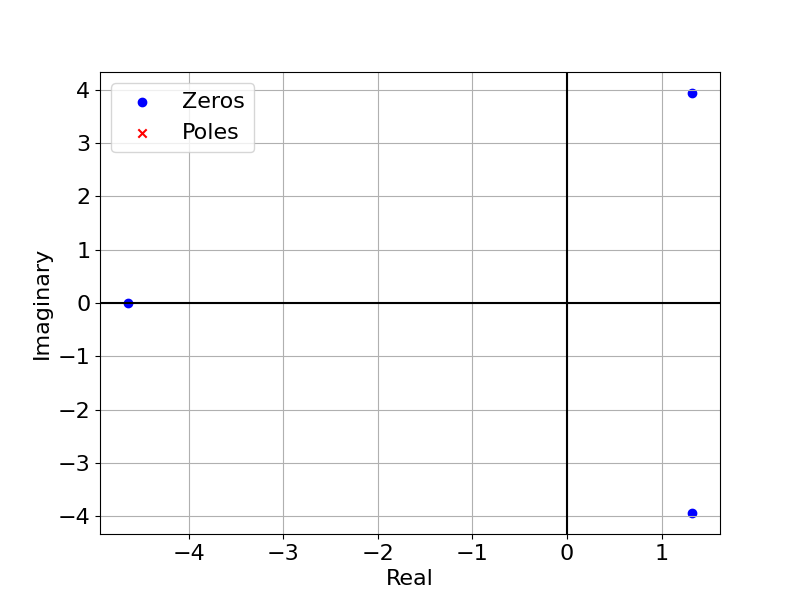
\includegraphics[width = \columnwidth]{2023/IN/24/figs/poles and root_plot.png}
  \caption{}
    \label{fig:graph1}
\end{figure}

% \bibliographystyle{IEEEtran}

\newpage

\item The circuit shown in the figure is initially in the steady state with the switch K in open condition and $\overline{K}$ in closed condition. The switch K is closed and $\overline{K}$ is opened simultaneously at the instant $t = t_1$, where $t_1 > 0$. The minimum value of $t_1$ in milliseconds such that there is no transient in the voltage across the 100 $\mu F$ capacitor, is \rule{1cm}{0.15mm} (Round off to 2 decimal places) \hfill (GATE EE 2023)
    \begin{circuitikz}[american]
        \draw (0,7) to [R=10$\Omega$] (0,2) to [short] (3.5,2) to [isource, l={$\sin\brak{1000t}$}] (3.5,7) to [short] (0,7);
        \draw (3.5,2) to [short] (5,2) to [short] (5,0) to [R=$10\Omega$] (7.5,0) to [battery2 = 5V] (10,0) to [short] (10,2) to [curved capacitor=100$\mu$F, invert] (10,7) to [short] (5,7) to [short] (3.5,7);
        \draw (5,2) to [short] (7, 2) to[ospst=$\overline{K}$] ++(1,0);
        \draw (5,5) to [short] (5,2);
        \draw (10,2) to [short] (8,2);
        \draw (5,7) to [short] (5,6) to[cspst=K] ++(0,-1) ;
\end{circuitikz}
\\
\solution
\iffalse
\documentclass[journal,12pt,twocolumn]{IEEEtran}
\usepackage{amsmath,amssymb,amsfonts,amsthm}
\usepackage{txfonts}
\usepackage{tkz-euclide}
\usepackage{listings}
\usepackage{gvv}
\usepackage[latin1]{inputenc}
\usepackage{adjustbox}
\usepackage{array}
\usepackage{tabularx}
\usepackage{pgf}
\usepackage{lmodern}
\usepackage{circuitikz}
\usepackage{tikz}
\usepackage{graphicx}

\begin{document}
\bibliographystyle{IEEEtran}

\vspace{3cm}

\title{}
\author{EE23BTECH11054 -  Sai Krishna Shanigarapu$^{*}$
}
\maketitle
\newpage
\bigskip

% \renewcommand{\thefigure}{\theenumi}
% \renewcommand{\thetable}{\theenumi}

\section*{Gate EE 2023}
54. \hspace{2pt}The circuit shown in the figure is initially in the steady state with the switch K in open condition and $\overline{K}$ in closed condition. The switch K is closed and $\overline{K}$ is opened simultaneously at the instant $t = t_1$, where $t_1 > 0$. The minimum value of $t_1$ in milliseconds such that there is no transient in the voltage across the 100 $\mu F$ capacitor, is \rule{1cm}{0.15mm} (Round off to 2 decimal places).\\ 
\hfill(GATE EE 2023)

\begin{figure}[ht]
  \centering
  \begin{adjustbox}{width=1\columnwidth}
          \begin{circuitikz}[american]
        \draw (0,7) to [R=10$\Omega$] (0,2) to [short] (3.5,2) to [isource, l={$\sin\brak{1000t}$}] (3.5,7) to [short] (0,7);
        \draw (3.5,2) to [short] (5,2) to [short] (5,0) to [R=$10\Omega$] (7.5,0) to [battery2 = 5V] (10,0) to [short] (10,2) to [curved capacitor=100$\mu$F, invert] (10,7) to [short] (5,7) to [short] (3.5,7);
        \draw (5,2) to [short] (7, 2) to[ospst=$\overline{K}$] ++(1,0);
        \draw (5,5) to [short] (5,2);
        \draw (10,2) to [short] (8,2);
        \draw (5,7) to [short] (5,6) to[cspst=K] ++(0,-1) ;
\end{circuitikz}

  \end{adjustbox}
  \caption{Circuit 1}
\end{figure}

\solution
\fi
\begin{enumerate}
\item Switch K is open and $\overline{K}$ is closed.

\begin{figure}[ht]
  \centering
          \begin{circuitikz}[american]
        \draw (0,7) to [R=10$\Omega$] (0,2) to [short] (3,2) to [isource, l=$1\angle{0^\circ}$] (3,7) to [short] (0,7);
        \draw (3,7) to [short, i=$I_1$] (7,7);
        \draw (3,2) to [short] (7,2);
        \draw (7,7) -- ++(0,-1.5)
        to [open, v=$V_1$, o-o] ++(0,-1.5) -- ++(0,-2);
\end{circuitikz}


  \caption{K is open and $\overline{K}$ is closed}
\end{figure}


Using Current divider rule,
\begin{align}
   I_1\brak{j\omega} &= \frac{10}{10+\frac{1}{j\omega C}}\\
   V_1\brak{j\omega} &= \frac{10}{1+10j\omega C}\\
   \abs{V_1\brak{j\omega}} &= 5\sqrt{2}
 \end{align}
 From Table \ref{tab:Gate.ee.54.1}
 \begin{align}
   V_1\brak{t} &= 5\sqrt{2}\sin\brak{\omega t - \frac{\pi}{4}} \label{eq:1.gate.ee.23.54}
\end{align}


\item Switch K is closed and $\overline{K}$ is open.


\begin{figure}[ht]
  \centering
      %\begin{circuitikz}[american]
        %\draw (0,0) to [R=10$\Omega$] (1.5,0) to [battery2=5V] (4,0);
        %\draw (0,0) to [short] (0,3) to [short] (4,3) to [C=100$\mu$F, %v=$V_c\brak{\infty}$] (4,0) ;
%\end{circuitikz}

\begin{circuitikz}[american]
    \draw (0,0) to [R=10$\Omega$] (1.5,0) to [battery2=$\frac{5}{s}$] (4,0);
    \draw[<-, thick] (1.5,1) arc (-90:90:0.5) node[midway, left] {$I(s)$};
    \draw (0,0) to [short] (0,3) to [short] (4,3) to [C=$\frac{10^4}{s}$, v=$V_c\brak{s}$] (4,0);
\end{circuitikz}


  \caption{K is closed and $\overline{K}$ is open}
\end{figure}
}


The capacitor is charged. Thus, acts as a voltage source.\\
From eq\brak{\ref{eq:1.gate.ee.23.54}} and Table \ref{tab:Gate.ee.54.2}
\begin{align}
    V_1\brak{s} &= \frac{5000 - 5s}{s^2 + 10^6} \\
    I\brak{s} &= \frac{\frac{5}{s} - V_1\brak{s}}{10 + \frac{10^4}{s}}\\
    V_c\brak{s} &= \frac{5}{s} - 10\brak{\frac{5-V_1\brak{s}}{1+10^{-3}s}}
\end{align}
\end{enumerate}

For transient analysis,
\begin{align}
    \frac{5-V_1\brak{s}}{1+10^{-3}s} &= 0\\
    \implies V_1\brak{s} &= 5\\
    \frac{10^7}{\brak{s^2+10^6}\brak{s+10^3}} &= \frac{5}{s}\\
    \frac{5}{s+10^3} + \frac{10^3-s}{s^2 + 10^6} &= \frac{5}{s}\\
    \frac{-s}{s^2+10^6} + \frac{10^3}{s^2 + 10^6} + \frac{1}{s+10^3} &= \frac{1}{s}
\end{align}
From Table \ref{tab:Gate.ee.54.2}
\begin{align}
    -\cos\brak{1000t_1}+\sin\brak{1000t_1}+e^{-10^3 t_1} &= 1\\
    \implies t_1 \approx 1.57\text{msec}
\end{align}

\begin{table}[ht]
       \setlength{\arrayrulewidth}{0.3mm}
\setlength{\tabcolsep}{20pt}
\renewcommand{\arraystretch}{1.3}



\begin{tabular}{|c|c|c|}
\hline

Parameter& Description & Remarks\\
\hline
$\omega$ & frequency of sine-wave & 1000 rad s$^{-1}$\\
\hline
$V_1\brak{t}$ & Voltage across capacitor & $\abs{V_1\brak{j\omega}}\sin\brak{\omega t - \angle{V_1\brak{j\omega}}}$\\
\hline
$\angle{V_1\brak{j\omega}} $ & phase of $V_1\brak{j\omega}$ & $\frac{-\pi}{4}$\\
\hline
$C$ & Capacitance & 100$\mu$F\\
\hline

\end{tabular}






    \caption{Parameters}
    \label{tab:Gate.ee.54.1}

\end{table}


\begin{table}[ht]
    \setlength{\arrayrulewidth}{0.3mm}
\setlength{\tabcolsep}{20pt}
\renewcommand{\arraystretch}{1.3}


\begin{tabular}{|c|c|}
\hline

S Domain & Time Domain\\
\hline
$\frac{1}{s}$ & $u\brak{t}$\\
\hline
$\frac{-s}{a^2+s^2}$ & $-\cos\brak{at}$\\
\hline
$\frac{a}{a^2+s^2}$ & $\sin\brak{at}$\\
\hline
$\frac{1}{s+a}$ & $e^{-at}$\\
\hline

\end{tabular}





    \caption{Laplace transforms}
    \label{tab:Gate.ee.54.2}
\end{table}

\begin{figure}[htbp]
    \centering
    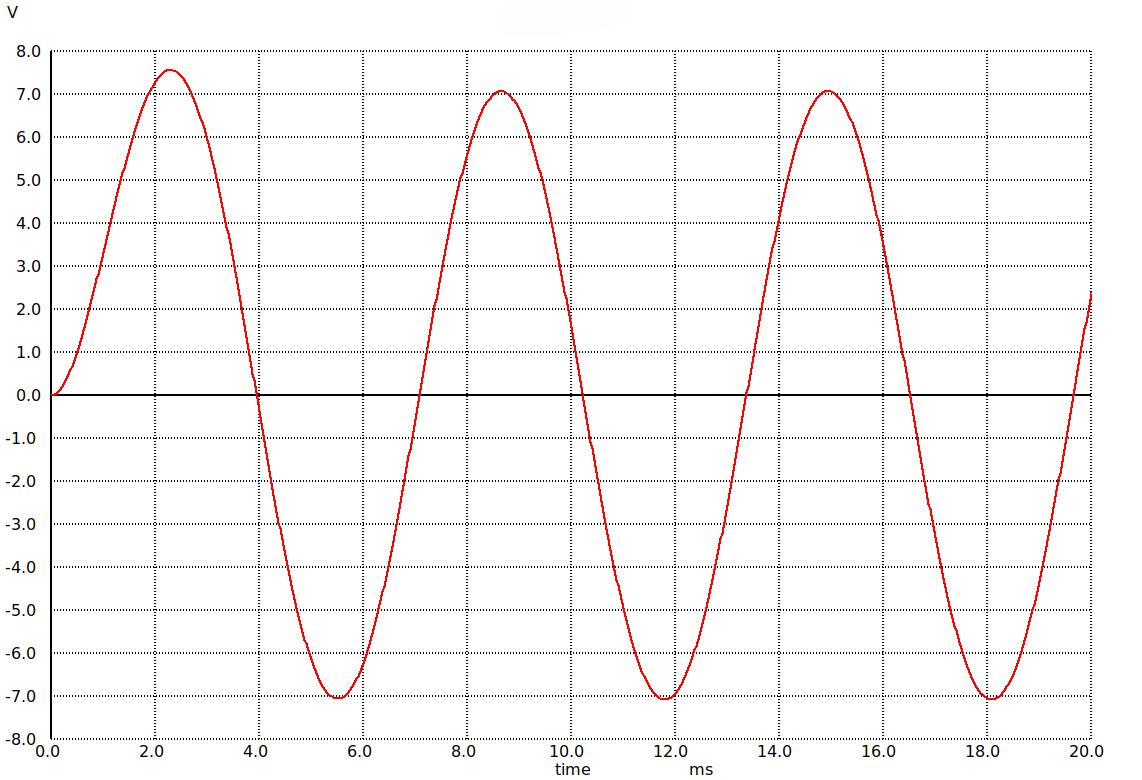
\includegraphics[width=1\columnwidth]{2023/EE/54/figs/fig1.png}
    \caption{plot of $V_1$ vs time}
\end{figure}

\begin{figure}[htbp]
    \centering
    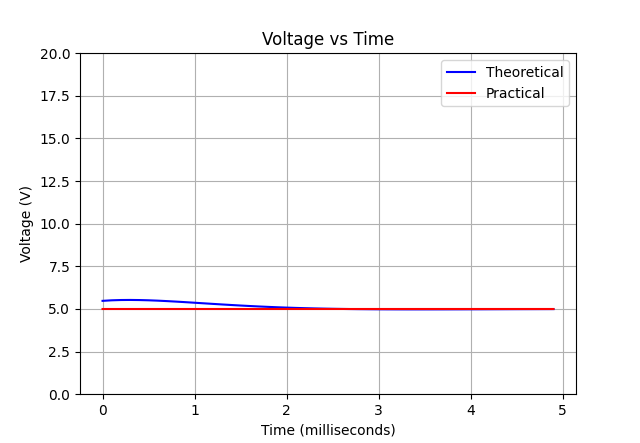
\includegraphics[width=1\columnwidth]{2023/EE/54/figs/fig3.png}
    \caption{plot of $V_c$ vs time}
\end{figure}

%\end{document}


\newpage
\item $y=e^{mx}+e^{-mx}$ is the solution of which differential equation?
\begin{enumerate}[label=\textbf{\arabic*.}, font=\bfseries, align=left]
    \item $\frac{dy}{dx} - my = 0$ 
    \item $\frac{dy}{dx} + my = 0$ 
    \item $\frac{d^{2}y}{dx^{2}} + m^{2}y = 0$ 
    \item $\frac{d^{2}y}{dx^{2}} - m^{2}y = 0$ 
\end{enumerate} \hfill(GATE AG 2023)
\solution

\newpage
\item  A cascade control strategy is shown in the figure below. The transfer function between the output $(y)$ and the secondary disturbance $(d_2)$ is defined as  \\
$$G_{d2}(s)= \frac{y(s)}{d_2(s)}$$. 
Which one of the following is the CORRECT expression for the transfer function $G_{d2}(s)$? \\
\begin{figure}[h]
    \centering
    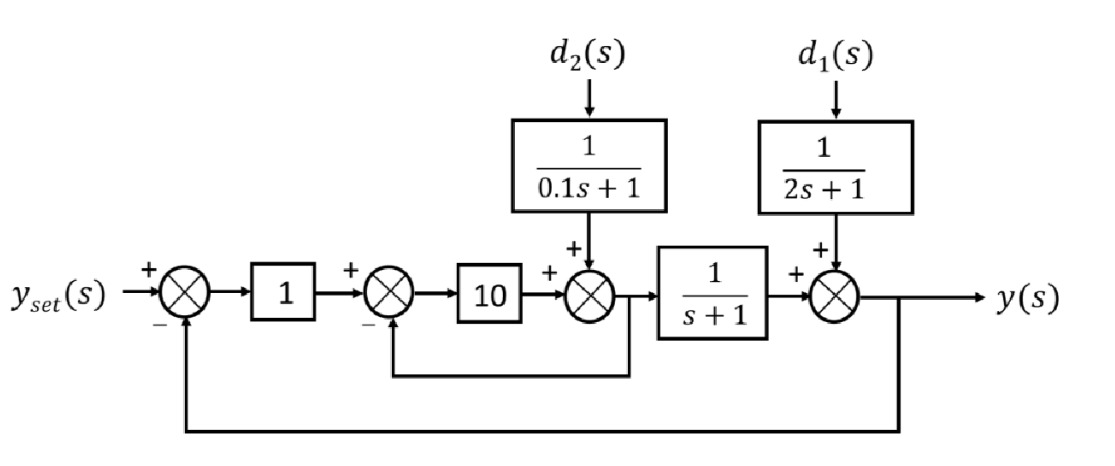
\includegraphics[scale=0.25]{2023/CH/44/figs/g44fig1.jpeg}
    \caption{ }
    \label{}
\end{figure}
\begin{enumerate}[label=\Alph*.]
\item $\frac{1}{(11s+21)(0.1s+1)}$ 
\item $\frac{1}{(s+1)(0.1s+1)}$
\item $\frac{(s+1)}{(s+2)(0.1s+1)}$
\item $\frac{(s+1)}{(s+1)(0.1s+1)}$
\end{enumerate} \hfill (GATE CH 2023)
\solution
\newpage
\item In the differential equation $\frac{dy}{dx} + \alpha x y = 0, \alpha$ is a positive constant. If $y = 1.0$ at
$x = 0.0$, and $y = 0.8$ at $x = 1.0$, the value of $\alpha$ is (rounded off to three decimal places).  \hfill(GATE CE 2023)
\solution

\newpage
\item The switch $S_1$ was closed and $S_2$ was open for a long time. At t=0,switch $S_1$ is opened and $S_2$ is closed,simultaneously. The value of $i_c(0^{+})$, in amperes, is . \hfill (GATE EC 2023)\\
\begin{circuitikz}[american]
   \draw (0,0) to [isource, l=1A] (0,4) ;
   \draw (0,0) to [short] (3,0) to [C = 0.01F] (3,4) to [short] (6,4) to [R = 100 $\Omega$] (6,2) to [L = 1H] (6,0) to [short] (9,0) to [R = 25 $\Omega$] (9,4) to [short] (6,4) ;
   \draw (3,0) to [short] (6,0) ;
   \draw (0,4) to [ospst = $S_1$] ++(3,0); 
   \draw (7.5,4) to [cspst = $S_2$] ++(0,-2);
   \draw (7.5,2) to [short] (6,2) ;
   \draw (3,4) to [short ,i = $i_c$] (3,3);
   
\end{circuitikz}

\newpage

\item The continuous time signal $x(t)$ is described by:
\begin{align}
x(t)=
    \begin{cases}
        1, & \text{if } 0\: {\displaystyle \leq }\:t\:{\displaystyle \leq }\:1\\
        0, & \text{elsewhere}
    \end{cases} 
\end{align}
If $y(t)$ represents $x(t)$ convolved with itself, which of the following options is/are TRUE?
\begin{enumerate}[label = \Alph*]
    \item $y(t)$ = 0 for all $t<0$\\
    \item $y(t)$ = 0 for all $t>1$\\
    \item $y(t)$ = 0 for all $t>3$\\
    \item $\int_{0.1}^{0.75} \frac{dy(t)}{dt}\: \text{dt} \neq 0$
\end{enumerate}
\solution
\newpage

\item The Z-transform of a discrete signal $x\brak{n}$ is
\begin{align}
X\brak{z}=\dfrac{4z}{\brak{z-\dfrac{1}{5}} \brak{z-\dfrac{2}{3}} \brak{z-3}} \text{ with ROC= }R
\end{align}
Which one of the following statements is TRUE?
\begin{enumerate}[label = (\alph*)]
     \item Discrete time Fourier transform of $x\sbrak{n}$ converges if $R$ is $|z|>3$\\
     \item Discrete time Fourier transform of $x\sbrak{n}$ converges if $ R$ is $\dfrac{2}{3}<|z|<3$\\
     \item Discrete time Fourier transform of $x\sbrak{n}$ converges if $R$ is such that $x\sbrak{n}$ is a left-sided sequence.\\
     \item Discrete time Fourier transform of $x\sbrak{n}$ converges if $R$ is such that $x\sbrak{n}$is a right-sided sequence.\\
 \end{enumerate} \hfill{GATE EE 2023}
 \solution
 \newpage
 
\item The phase margin of the transfer function $G(s) = \frac{2(1-s)}{(1+s)^2}$ is \rule{1cm}{0.15mm} degrees. (rounded off to the nearest integer). \hfill (GATE IN 2023)\\
\solution
\iffalse
\let\negmedspace\undefined
\let\negthickspace\undefined
\documentclass[journal,12pt,twocolumn]{IEEEtran}
\usepackage{cite}
\usepackage{amsmath,amssymb,amsfonts,amsthm}
\usepackage{algorithmic}
\usepackage{graphicx}
\usepackage{textcomp}
\usepackage{xcolor}
\usepackage{txfonts}
\usepackage{listings}
\usepackage{enumitem}
\usepackage{mathtools}
\usepackage{gensymb}
\usepackage{comment}
\usepackage[breaklinks=true]{hyperref}
\usepackage{tkz-euclide} 
\usepackage{listings}
\usepackage{gvv}                                        
\def\inputGnumericTable{}                                 
\usepackage[latin1]{inputenc}                                
\usepackage{color}                                            
\usepackage{array}                                            
\usepackage{longtable}                                       
\usepackage{calc}                                             
\usepackage{multirow}                                         
\usepackage{hhline}                                           
\usepackage{ifthen}                                           
\usepackage{lscape}
\newtheorem{theorem}{Theorem}[section]
\newtheorem{problem}{Problem}
\newtheorem{proposition}{Proposition}[section]
\newtheorem{lemma}{Lemma}[section]
\newtheorem{corollary}[theorem]{Corollary}
\newtheorem{example}{Example}[section]
\newtheorem{definition}[problem]{Definition}
\newcommand{\BEQA}{\begin{eqnarray}}
\newcommand{\EEQA}{\end{eqnarray}}
\newcommand{\define}{\stackrel{\triangle}{=}}
\theoremstyle{remark}
\newtheorem{rem}{Remark}
\begin{document}

\bibliographystyle{IEEEtran}
\vspace{3cm}

\title{GATE: IN - 50.2023}
\author{EE23BTECH11224 - Sri Krishna Prabhas Yadla$^{*}$% <-this % stops a space
}
\maketitle
\newpage
\bigskip

\renewcommand{\thefigure}{\arabic{figure}}
\renewcommand{\thetable}{\arabic{table}}


\vspace{3cm}
\textbf{Question:} The phase margin of the transfer function $G(s) = \frac{2(1-s)}{(1+s)^2}$ is \rule{1cm}{0.15mm} degrees. (rounded off to the nearest integer). \hfill (GATE IN 2023)\\
\solution
\fi
\begin{table}[htbp]
	\centering
	\def\arraystrech{1.5}
	\begin{tabular}{|c|c|}
\hline
\textbf{Parameters} & \textbf{Description} \\
\hline
$\omega_c$ & crossover frequency \\
\hline
$\angle G(j\omega)$ & phase angle of the transfer function \\
\hline
$PM$ & $\angle G(j\omega_c)+180\degree$; Phase Margin\\
\hline
\end{tabular}

	\caption{Parameters}
	\label{tab:parameters}
\end{table}
\newline
Considering $s=j\omega$,
\begin{align}
	G(j\omega) &= \frac{2(1-j\omega)}{(1+j\omega)^2} \\
	&= \frac{2(1-j\omega)^3}{\abs{1+j\omega}^4}\\
	&= \frac{2}{(1+\omega^2)^2}(1-j\omega)^3 \\
	&= \frac{2}{\sqrt{1+\omega^2}}(e^{-j\omega})^3 \\
	\implies \abs{G(j\omega)} &= \frac{2}{\sqrt{1+\omega^2}} \\
	\implies \angle G(j\omega) &= 3\tan^{-1}(-\omega)
\end{align}
At $\omega = \omega_c$, $Gain = 0$
\begin{align}
	\implies \abs{G(j\omega_c)} &= 1 \\
	\frac{2}{\sqrt{1+\omega_c^2}} &= 1 \\
	\implies \omega_c &= \sqrt{3} \\
	\angle G(j\omega_c) &= 3\tan^{-1}(-\sqrt{3}) \\
	&= -180\degree
\end{align}
From \tabref{tab:parameters},
\begin{align}
	PM &= 0\degree
\end{align}
\begin{figure}[htbp]
	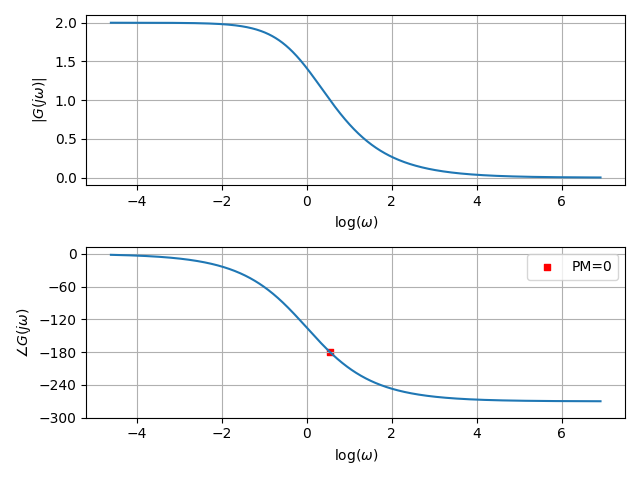
\includegraphics[width=\columnwidth]{2023/IN/50/figs/bode.png}
	\caption{Bode Plot of Transfer Function $G(s)$}
	\label{fig:bode}
\end{figure}

\newpage
\item Consider the second-order linear differential equation
\[x^2\frac{d^2y}{dx^2}+x\frac{dy}{dx}-y=0, \; x\geq 1\]
with the initial conditions \[y(x=1)=6,\; \;\; \frac{dy}{dx}\big{|}_{x=1}=2.\]
Then the value of $y$ at $x=2$ is \rule{2cm}{0.1mm}.\\{\hfill{GATE ME 2023}}\\
\solution
\newpage
\item The transfer function of a measuring instrument is \\
$$G_m(s) = \frac{1.05}{2s+1}exp(-s)$$
At time $t = 0$, a step change of +1 unit is introduced in the input of this instrument.The time taken by the instrument to show an increase of 1 unit in its output is(rounded off to two decimal places).\\ \hfill (GATE CH 2023)
\solution
\item
The laplace transform of $x_1(t)$ = $e^{-t}u(t)$ is $X_1(s)$, where $u(t)$ is the unit step function. The laplace transform of $x_2(t) = e^tu(-t)$ is $X_2(s)$. Which one of the following statements is TRUE?
\begin{enumerate}
    \item The region of convergence of $X_1(s)$ is $Re(s) \geq 0$
    \item The region of convergence of $X_2(s)$ is confined to the left half-plane of s.
    \item The region of convergence of $X_1(s)$ is confined to the right half-plane of s.
    \item the imaginary axis in the s-plane is included in both the region of convergence of $X_1(s)$ and the region of convergence of $X_2(s)$.
\end{enumerate} \hfill(GATE BM 2023)\\
\solution
\iffalse
\let\negmedspace\undefined
\let\negthickspace\undefined
\documentclass[journal,12pt,onecolumn]{IEEEtran}
\usepackage{cite}
\usepackage{amsmath,amssymb,amsfonts,amsthm}
\usepackage{algorithmic}
\usepackage{graphicx}
\usepackage{textcomp}
\usepackage{xcolor}
\usepackage{txfonts}
\usepackage{listings}
\usepackage{enumitem}
\usepackage{mathtools}
\usepackage{gensymb}
\usepackage{comment}
\usepackage[breaklinks=true]{hyperref}
\usepackage{tkz-euclide} 
\usepackage{listings}
\usepackage{gvv}    
\usepackage{enumitem}
\usepackage{amsmath}
\def\inputGnumericTable{}                                 
\usepackage[latin1]{inputenc}                                
\usepackage{color}                                            
\usepackage{array}                                            
\usepackage{longtable}                                       
\usepackage{calc}                                             
\usepackage{multirow}                                         
\usepackage{hhline}                                           
\usepackage{ifthen}                                           
\usepackage{lscape}
\usepackage{tabularx}

\newtheorem{theorem}{Theorem}[section]
\newtheorem{problem}{Problem}
\newtheorem{proposition}{Proposition}[section]
\newtheorem{lemma}{Lemma}[section]
\newtheorem{corollary}[theorem]{Corollary}
\newtheorem{example}{Example}[section]
\newtheorem{definition}[problem]{Definition}
\newcommand{\BEQA}{\begin{eqnarray}}
\newcommand{\EEQA}{\end{eqnarray}}
\newcommand{\define}{\stackrel{\triangle}{=}}
\theoremstyle{remark}
\newtheorem{rem}{Remark}
\begin{document}
\bibliographystyle{IEEEtran}
\vspace{3cm}

\title{GATE-BM-39.2023: }
\author{EE23BTECH11025 - Anantha Krishnan $^{}$% <-this % stops a space
}
\maketitle
\bigskip



\section{question}

The laplace transform of $x_1(t)$ = $e^{-t}u(t)$ is $X_1(s)$, where $u(t)$ is the unit step function. The laplace transform of $x_2(t) = e^tu(-t)$ is $X_2(s)$. Which one of the following statements is TRUE?
\begin{enumerate}
    \item The region of convergence of $X_1(s)$ is $Re(s) \geq 0$
    \item The region of convergence of $X_2(s)$ is confined to the left half-plane of s.
    \item The region of convergence of $X_1(s)$ is confined to the right half-plane of s.
    \item the imaginary axis in the s-plane is included in both the region of convergence of $X_1(s)$ and the region of convergence of $X_2(s)$.
\end{enumerate}
 



\textbf{Solutions :}
\fi
\begin{table}[ht!]
\centering
\begin{tabular}{ |c|c| } 
 \hline
Symbols & Description \\
\hline
 $X_1(s)$ & Laplace transform of $x_1(t)$ \\
 \hline
 $X_2(s)$ & Laplace transform of $x_2(t)$\\
\hline
 $u(t)$ & Unit step function\\
\hline
\end{tabular}
\caption{Parameters, Descriptions}
\label{table:ee25-tab2}
\end{table}




    \begin{enumerate}
        \item 
Laplace transform of $x_1(t)$ is given by :
\begin{align}
    X_1(s) &=  \int_{-\infty}^{\infty} e^{-t}e^{-st}u(t) \,dt
    \end{align}
    Let $s=\sigma+j\omega$ :
\begin{align}
 X_1(s) &= \int_{0}^{\infty}e^{-t\brak{\sigma+1}}e^{-tj\beta} \,dt\\
       &=  \left[\frac{-e^{-t\brak{\sigma+1}}e^{-tj\beta}}{\brak{\sigma+1}+j\beta}\right]_{0}^{\infty}  
       \end{align}
        For $X_1(s)$ to be convergent,$\quad\abs{-e^{-t\brak{\sigma+1}}e^{-tj\beta}}$ must converge $\forall t \epsilon \brak{0,\infty}$, so:
        \begin{align}
\quad\abs{e^{-tj\beta}} = \abs{1}, \forall \beta \epsilon \mathbb{R} \implies Im\brak{s} \epsilon \mathbb{R}\\
\sigma + 1 > 0 \implies  \Re\brak{s}>-1   
        \end{align}
Putting the limits :
       \begin{align}
X_1(s)&= \frac{1}{s+1} , \Re\brak{s} > -1 
\end{align}
\item  
Laplace transform of $x_2(t)$ is given by :
\begin{align}
    X_2(s) &=  \int_{-\infty}^{\infty} e^{t}e^{-st}u(-t) \,dt
        \end{align}
    Let $s=\sigma+j\omega$ :
\begin{align}
    &= \int_{-\infty}^{0}e^{t\brak{1-\sigma}}e^{-tj\beta} \,dt\\
      &=  \left[\frac{e^{t\brak{1-\sigma}}e^{-tj\beta}}{\brak{1-\sigma}-j\beta}\right]_{-\infty}^{0}  
     \end{align}
      For $X_2(s)$ to be convergent,$\quad\abs{e^{t\brak{1-\sigma}}e^{-tj\beta}}$ must converge $\forall t\epsilon\brak{-\infty,0}$, so:
     \begin{align}
\quad\abs{e^{-tj\beta}} = \abs{1}, \forall \beta \epsilon \mathbb{R} \implies Im\brak{s} \epsilon \mathbb{R}\\
1-\sigma > 0 \implies  \Re\brak{s} < 1 
        \end{align}
Putting the limits 
     \begin{align}
            X_2(s)&= \frac{1}{1-s} , \Re\brak{s} < 1
\end{align}
\begin{figure}[h!]
\begin{center}
    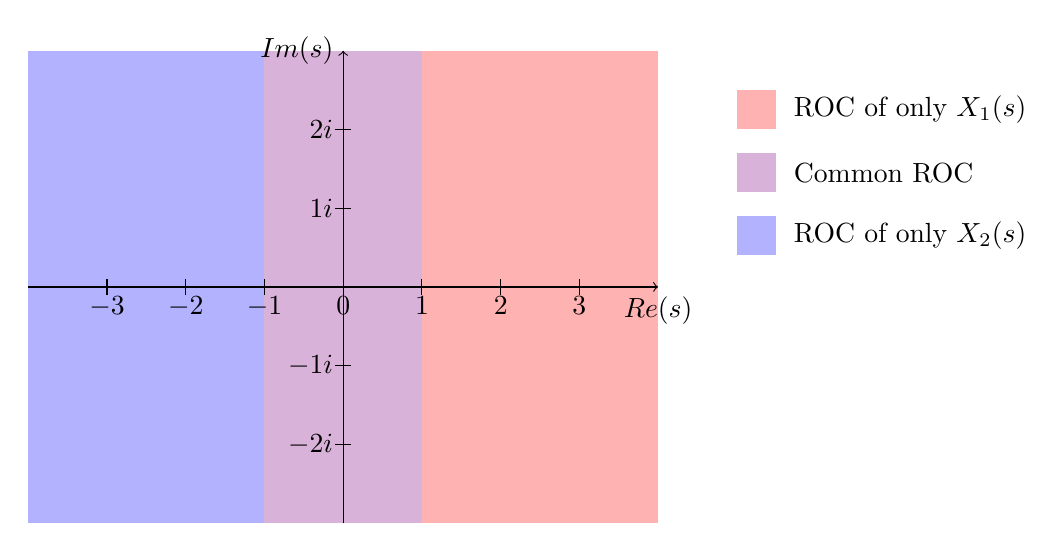
\begin{tikzpicture}
    \fill[red!30] (1,-3) rectangle (4,3);
    \fill[violet!30] (-1,-3) rectangle (1,3);
    \fill[blue!30] (-4,-3) rectangle (-1,3);
    % Axis length
    \draw[->] (-4,0) -- (4,0) node[below] {$\text{Re}(s)$};
    \draw[->] (0,-3) -- (0,3) node[left] {$\text{Im}(s)$};
    % X-axis
    \foreach \x in {-3,-2,-1,0,1,2,3}
        \draw (\x,-0.1) -- (\x,0.1) node[below=3pt] {$\x$};
    % Y-axis
    \foreach \y in {-2,-1,1,2}
        \draw (-0.1,\y) -- (0.1,\y) node[left=3pt] {$\y i$};
    % Legend
    \begin{scope}[shift={(5,2)}]
        \fill[red!30] (0,0) rectangle ++(0.5,0.5);
        \node[right] at (0.6,0.25) {ROC of only $X_1(s)$};
        \fill[violet!30] (0,-0.8) rectangle ++(0.5,0.5);
        \node[right] at (0.6,-0.55) {Common ROC};
        \fill[blue!30] (0,-1.6) rectangle ++(0.5,0.5);
        \node[right] at (0.6,-1.35) {ROC of only $X_2(s)$};
    \end{scope}
\end{tikzpicture}
\caption{Representation of ROCs of $X_1(s)$ and $X_2(s)$} \label{fig:ee23-b1}
\end{center}
\end{figure}


Based on the overlap of regions of convergence of  $X_1(s)$ and $X_2(s)$ from \ref{fig:ee23-b1} , we can conclude that option 4) is correct .  
    \end{enumerate}








\newpage
\item Given that $\frac{dy}{dx}=2x+y$ and $y=1$,when $x=0$ Using Runge-Kutta fourth order method,the value of $y$ at $x=0.2$ is \hfill(GATE 2023 AG 50) \\
\solution

\item The magnitude and phase plots shown in the figure match with the transfer-
function
\begin{figure}[h]
    \centering
    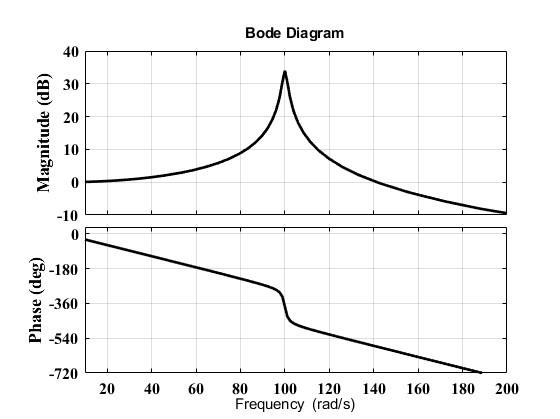
\includegraphics[width=\columnwidth]{2023/IN/43/figs/question.png}
\end{figure}\\
\begin{enumerate}
\item $\frac{10000}{s^2+2s+10000}$\\
\item $\frac{10000}{s^2+2s+10000}e^{-0.05s}$\\
\item $\frac{10000}{s^2+2s+10000}e^{-0.5\times10^{-12}s}$\\
\item $\frac{100}{s^2+2s+100}$
\end{enumerate}
\hfill{(GATE IN 2023)}
\solution

\newpage
\item The Laplace transform of the continuous-time signal $x\brak{t} = e^{-3t}u\brak{t - 5}$ is 
\rule{1cm}{0.15mm}, where $u\brak{t}$ denotes the continuous-time unit step signal.

\begin{enumerate}[label = \Alph*)]
    \item $\frac{e^{-5s}}{s + 3}$, Real$\{s\} > -3$\\
    \item $\frac{e^{-5(s - 3)}}{s - 3}$, Real$\{s\} > 3$\\
    \item $\frac{e^{-5(s + 3)}}{s + 3}$, Real$\{s\} > -3$\\
    \item $\frac{e^{-5(s - 3)}}{s + 3}$, Real$\{s\} > -3$\\
\end{enumerate}
\solution
\iffalse
\let\negmedspace\undefined
\let\negthickspace\undefined
\documentclass[journal,12pt,twocolumn]{IEEEtran}
\usepackage{cite}
\usepackage{amsmath,amssymb,amsfonts,amsthm}
\usepackage{algorithmic}
\usepackage{graphicx}
\usepackage{textcomp}
\usepackage{xcolor}
\usepackage{txfonts}
\usepackage{listings}
\usepackage{enumitem}
\usepackage{mathtools}
\usepackage{gensymb}
\usepackage{comment}
\usepackage[breaklinks=true]{hyperref}
\usepackage{tkz-euclide} 
\usepackage{listings}
\usepackage{gvv}                                        
\def\inputGnumericTable{}                                 
\usepackage[latin1]{inputenc}                                
\usepackage{color}                                            
\usepackage{array}                                            
\usepackage{longtable}                                       
\usepackage{calc}                                             
\usepackage{multirow}                                         
\usepackage{hhline}                                           
\usepackage{ifthen}                                           
\usepackage{lscape}
\usepackage[center]{caption} % center the captions to figure

\newtheorem{theorem}{Theorem}[section]
\newtheorem{problem}{Problem}
\newtheorem{proposition}{Proposition}[section]
\newtheorem{lemma}{Lemma}[section]
\newtheorem{corollary}[theorem]{Corollary}
\newtheorem{example}{Example}[section]
\newtheorem{definition}[problem]{Definition}
\newcommand{\BEQA}{\begin{eqnarray}}
\newcommand{\EEQA}{\end{eqnarray}}
\newcommand{\define}{\stackrel{\triangle}{=}}
\theoremstyle{remark}
\newtheorem{rem}{Remark}
\begin{document}

\newcolumntype{M}[1]{>{\centering\arraybackslash}m{#1}}
\newcolumntype{N}{@{}m{0pt}@{}}

\bibliographystyle{IEEEtran}
\vspace{3cm}

\title{GATE 2023 IN 37Q} 
\author{ee23btech11223 - Soham Prabhakar More% <-this % stops a space
}
\maketitle
\newpage
\bigskip

\renewcommand{\thefigure}{\theenumi}
\renewcommand{\thetable}{\theenumi}

\bibliographystyle{IEEEtran}

\textbf{Question:} The Laplace transform of the continuous-time signal $x\brak{t} = e^{-3t}u\brak{t - 5}$ is 
\rule{1cm}{0.15mm}, where $u\brak{t}$ denotes the continuous-time unit step signal.

\solution
\fi

\begin{table}[ht]
    \begin{tabular}{|c|c|c|} 
    \hline
    \textbf{Variable} & \textbf{Description} & \textbf{Value} \\
    \hline
    $x(t)$ & input function & none \\
    \hline
    $y(t)$ & output function & $\sin(\pi t)$ \\
    \hline
    $H(s)$ & Transfer-function & $\frac{s-\pi}{s+\pi}$ \\
    \hline
\end{tabular}

\end{table}    

\begin{align}
    e^{-3t}u\brak{t} \system{L} \frac{1}{s + 3} \quad \Re\brak{s} > -3 \label{eq:2023.in.37.exp}
\end{align}
Using time shifting,
\begin{align}
    e^{-3(t - 5)}u\brak{t - 5} &\system{L} \frac{e^{-5s}}{s + 3} \\
    e^{-15}e^{-3(t - 5)}u\brak{t - 5} &\system{L} e^{-15}\frac{e^{-5s}}{s + 3} \\
    e^{-3t}u\brak{t - 5} &\system{L} \frac{e^{-5(s + 3)}}{s + 3} \\
    \therefore x\brak{t} &\system{L} \frac{e^{-5(s + 3)}}{s + 3} \quad \Re\brak{s} > -3
\end{align}

\begin{figure}[h!]
    \renewcommand\thefigure{3}
    \centering
    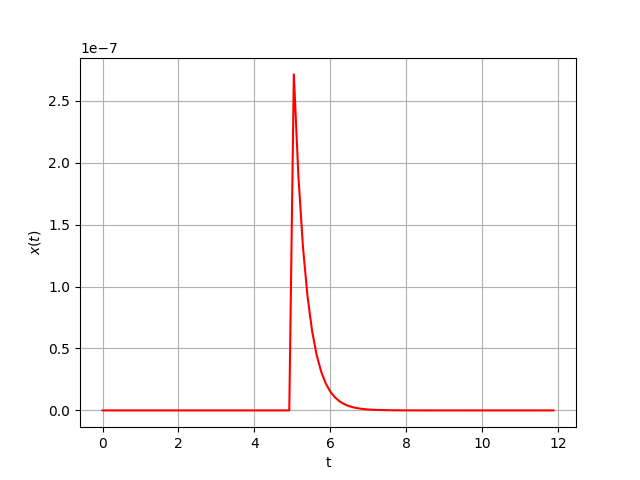
\includegraphics[width=\columnwidth]{figs/x_t.png}
    \caption[short]{Plot of $x\brak{t}$ vs $t$. See \tabref{Table:1}}
    \label{fig:2023.in.37.img1}
\end{figure}

%\end{document}



\newpage
\item The solution $ x(t) ,t \geq 0, $ to the differential equation
$ \ddot{x} = -k\dot{x}  , k > 0 $ with initial conditions $ x(0) = 1 $ and $ x\dot{o}(0) $ = 0 is\\
\solution
\pagebreak
\item  Consider the differential equation
\begin{align}
x^2\frac{d^2y}{dx^2} + 4x\frac{dy}{dx} + 2y = 0 \quad \text{for } x\geq 1 \nonumber
\end{align}
with initial conditions $y=0$ and $\frac{dy}{dx} = 1$ at
$x = 1$. The value of $y$ at $x = 2$ is ?\\

\hfill(GATE AE 2023)
\solution
\pagebreak

\item The time-dependent growth of a bacterial population is governed by the equation
\begin{align}
    \frac{dx}{dt}=x\brak{1-\frac{x}{200}}
\end{align}
where $x$ is the population size at time $t$. The initial population size is $x_0=100$
at $x=0$. As $t \rightarrow \infty$, the population size of bacteria asymptotically approaches
\begin{enumerate}[label=(\alph*)]
    \item $150$
    \item $200$
    \item $300$
    \item $500$
\end{enumerate}
\hfill{(GATE BM 2023)}
\solution
\newpage

\item Consider a lead compensator of the form \\
$K(s) = \frac{1 + \frac{s}{a}}{1 + \frac{s}{\beta a}}, \quad \beta > 1, \quad a > 0$\\
The frequency at which this compensator produces maximum phase lead is \(4 \, \text{rad/s}\). At this frequency, the gain amplification provided by the controller, assuming an asymptotic Bode-magnitude plot of \(K(s)\), is \(6 \, \text{dB}\). The values of \(a\) and \(\beta\), respectively, are
\begin{enumerate}
    \item $ 1, 16 $\\
    \item $\ 2, 4 $\\
    \item $ 3, 5 $\\
    \item $ 2.66, 2.25$\\
\end{enumerate}\hfill{(GATE EC 2023)}
\solution
\newpage

\item Second order ordinary differential equation $\frac{d^2y}{dx^2}-\frac{dy}{dx}-2y=0$ has values 
$y=2$ and$\frac{dy}{dx}=1$ at $x=0$.The value of $y$ at $x=1$ is?($round\; off\;\: to\;\: three\;\: decimal\;\: places$)
 \\ \hfill[GATE-ES 2023]\\
 \solution
 \newpage

 \item A continuous-time system that is initially at rest is described by,	
	\begin{center}
		$\dfrac{dy(t)}{dt} + 3y(t) = 2x(t)$
	\end{center}
where $x(t)$ is the input voltage and $y(t)$ is the output voltage.\\ 
The impulse response of the system is?
\hfill(GATE 2023 EE)
\solution
\newpage

\item Consider the equation $\frac{dy}{dx}+ay=\sin{\omega x}$,where $a$ and $\omega$ are constants.Given $y=1$ at $x=0$, correct all the correct statement(s) from the following as $x\to \infty$.
\begin{enumerate}

  \item[(A)]  $y \to 0$ if $a \neq 0$ \\ 
  \item[(B)]  $y \to 1$ if $a = 0$\\
  \item[(C)]  $y \to Aexp(|a|x)$ if $a < 0$; A is constant\\
  \item[(D)]  $y \to B \sin(\omega x+C)$ if $a>0$; B and C are constants\\
\end{enumerate}
\hfill(GATE AE 2023)
\solution
\newpage


\item \textbf{Question }:
The position $x(t)$ of a particle, at constant $\omega$, is described by the equation
\begin{align}
\frac{{d^2x}}{{dt^2}} = -\omega^2 x.
\end{align}
The initial conditions are $x(t=0)=1$ and $\frac{{dx}}{{dt}}\bigg|_{t=0}=0$. 
The position of the particle at $t=\frac{{3\pi}}{{\omega}}$ is \underline{\hspace{2cm}} (in integer).
\hfill{(GATE CH 2023)}
\solution
\newpage

\item \textbf{Question}:The initial value problem
$\frac{dy}{dt}+2y=0, y(0)=1 $
is solved numerically using the forward Euler's method with a constant and positive time step of $\delta $.\\
Let $y_n$ represent the numerical solution obtained after $n$ steps. The condition $\abs{y_{n+1}} \leq \abs{y_n}$is satisfied if and only if $\delta$ does not exceed \\
\hfill{(GATE ME 2023)}
\solution
\newpage

\item In the context of signals and systems, determine the phase cross-over frequency of the open-loop transfer function
\[
G(s) = \frac{k \cdot s \cdot (1+sT_1) \cdot (1+sT_2)}{s}
\]
with positive constants $k, T_1, T_2$ are positive constants.The phase crossover fequency,in rad/s,is
\begin{enumerate}
  \item[(a)] $\frac{1}{\sqrt{T_1 T_2}}$
  \item[(b)] $\frac{1}{T_1 T_2}$
  \item[(c)] $\frac{1}{T_1\sqrt{T_2}}$
  \item[(d)] $\frac{1}{\sqrt{T_2}T_1}$
\end{enumerate}
\hfill{(GATE EC 2023)}
\solution
\newpage

\end{enumerate}

\backmatter
\appendix
\iffalse
\chapter{ Convolution}
\chapter{ Z-transform}
\fi
\latexprintindex

\end{document}

 
